%%%%%%%%%%%%%%%%%%%%%%%%%%%%%%%%%%%%%%%%%%%%%%%%%%%%%%
% A Beamer template for University of Wollongong     %
% Based on THU beamer theme                          %
% Author: Qiuyu Lu                                   %
% Date: July 2024                                    %
% LPPL Licensed.                                     %
%%%%%%%%%%%%%%%%%%%%%%%%%%%%%%%%%%%%%%%%%%%%%%%%%%%%%%
% Customized for Sharif University of Technology     %
%%%%%%%%%%%%%%%%%%%%%%%%%%%%%%%%%%%%%%%%%%%%%%%%%%%%%%


\documentclass[default, aspectratio=169]{beamer}
%\documentclass[default]{beamer}  % for 4:3 ratio
\usepackage[T1]{fontenc} 
\usepackage{fourier} % see "http://faq.ktug.org/wiki/uploads/MathFonts.pdf" for other options
\usepackage{hyperref}
\usepackage{latexsym,amsmath,xcolor,multicol,booktabs,calligra}
\usepackage{graphicx,pstricks,listings,stackengine}
\usepackage{lipsum}
\usepackage{tikz}

\usepackage{pgffor}


\author{Ali Sharifi-Zarchi}
\title{Machine Learning (CE 40717)}
\subtitle{Fall 2024}
\institute{
	CE Department \\
	Sharif University of Technology
}
%\date{\small \today}
% \usepackage{UoWstyle}
\usepackage{SUTstyle}
\usepackage{amsmath}
\usepackage{amssymb}

%\usepackage{multicol}

% defs
\def\cmd#1{\texttt{\color{red}\footnotesize $\backslash$#1}}
\def\env#1{\texttt{\color{blue}\footnotesize #1}}
\definecolor{deepblue}{rgb}{0,0,0.5}
\definecolor{deepred}{RGB}{153,0,0}
\definecolor{deepgreen}{rgb}{0,0.5,0}
\definecolor{halfgray}{gray}{0.55}

\lstset{
	basicstyle=\ttfamily\small,
	keywordstyle=\bfseries\color{deepblue},
	emphstyle=\ttfamily\color{deepred},    % Custom highlighting style
	stringstyle=\color{deepgreen},
	numbers=left,
	numberstyle=\small\color{halfgray},
	rulesepcolor=\color{red!20!green!20!blue!20},
	frame=shadowbox,
}

\begin{document}
	
	
	
	\begin{frame}
		\titlepage
		\vspace*{-0.6cm}
		\begin{figure}[htpb]
			\begin{center}
				
\includegraphics[keepaspectratio, scale=0.25]{pic/sharif-main-logo.png}
			\end{center}
		\end{figure}
	\end{frame}
	
	\begin{frame}    
		\tableofcontents[sectionstyle=show,
		subsectionstyle=show/shaded/hide,
		subsubsectionstyle=show/shaded/hide]
	\end{frame}
	 \section{Motivation}
	\begin{frame}{How Do Humans See?}
		
		How can we enable computers to \textbf{see}?
		\begin{center}
			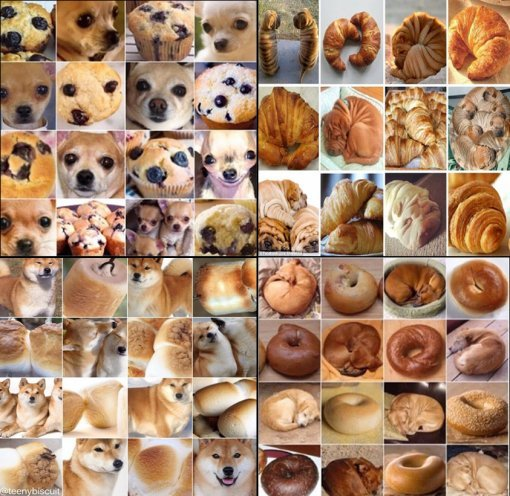
\includegraphics[keepaspectratio, scale=0.334]{pic/how.png}
			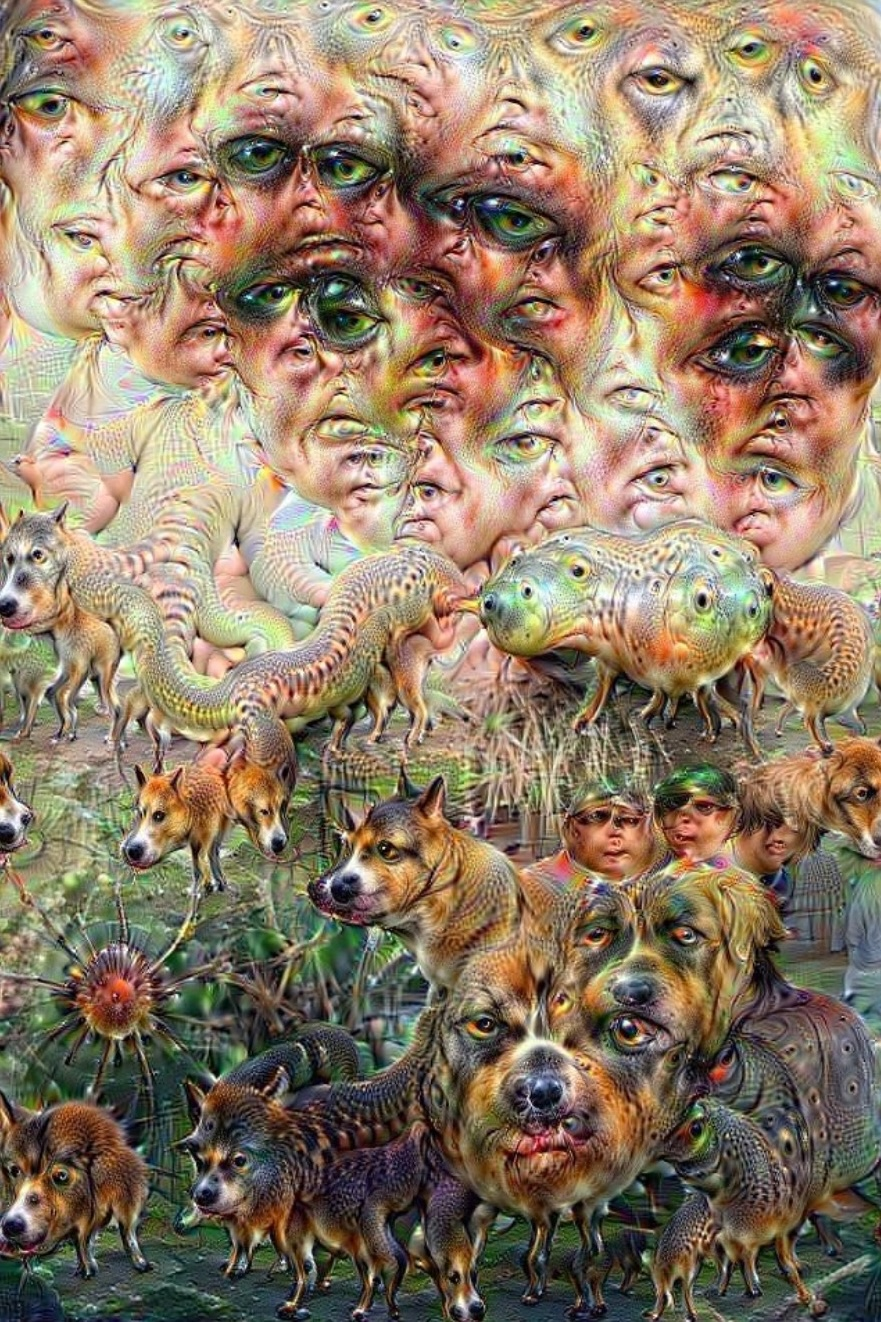
\includegraphics[keepaspectratio, scale=0.25]{pic/nothing.PNG}
		\end{center}
		\vfill
		\begin{tikzpicture}[remember picture,overlay]
			\node[anchor=south west, xshift=0.5cm, yshift=0.5cm] at (current page.south west) {
				\scriptsize Figure adapted from [4]
			};
		\end{tikzpicture}
		
	\end{frame}
	
	\begin{frame}{What Computers \textbf{See}: Images As Numbers}
		
		\begin{flushleft}
			{\textbf{An image is just a matrix} of numbers .i.e., $1080 \times 1080 \times 3$ for an RGB image.\\
				\textbf{Question}: is this Lincoln? Washington? Jefferson? Obama?\\
				How can the computer answer this question?}
			
			
		\end{flushleft}
		\centering
		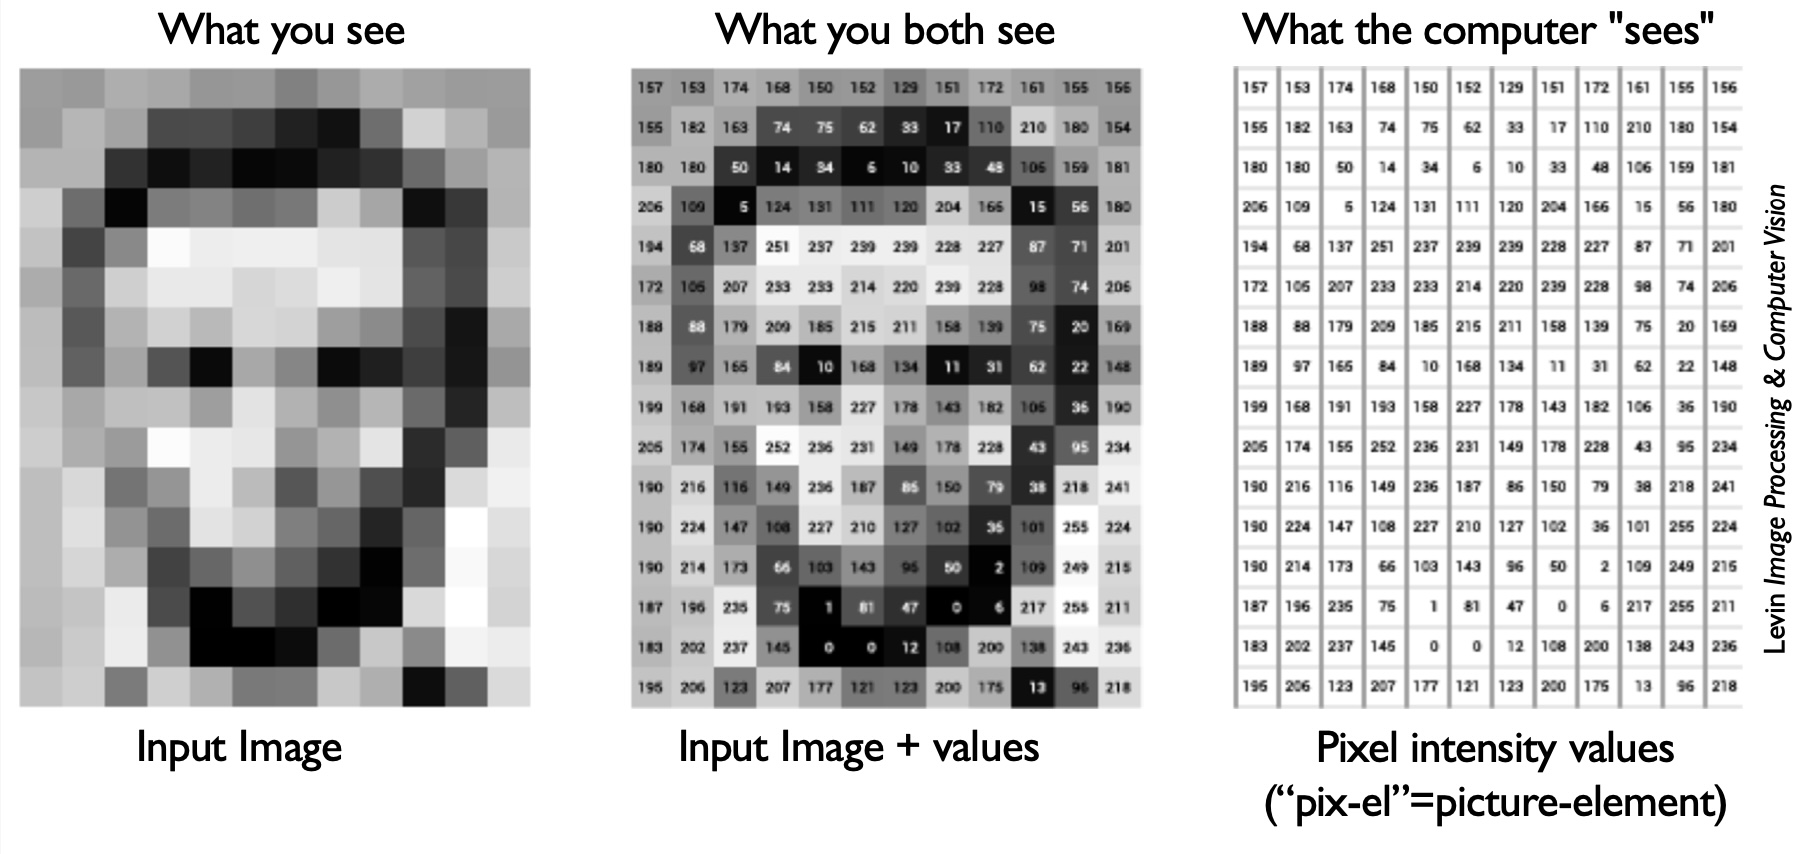
\includegraphics[keepaspectratio, scale=0.35]{pic/what.png}
		
		\begin{tikzpicture}[remember picture,overlay]
			\node[anchor=south west, xshift=0.5cm, yshift=0.5cm] at (current page.south west) {
				\scriptsize Figure adapted from [4]
			};
		\end{tikzpicture}
	\end{frame}
	\begin{frame}{What Is Computer Vision?}
		\centering
		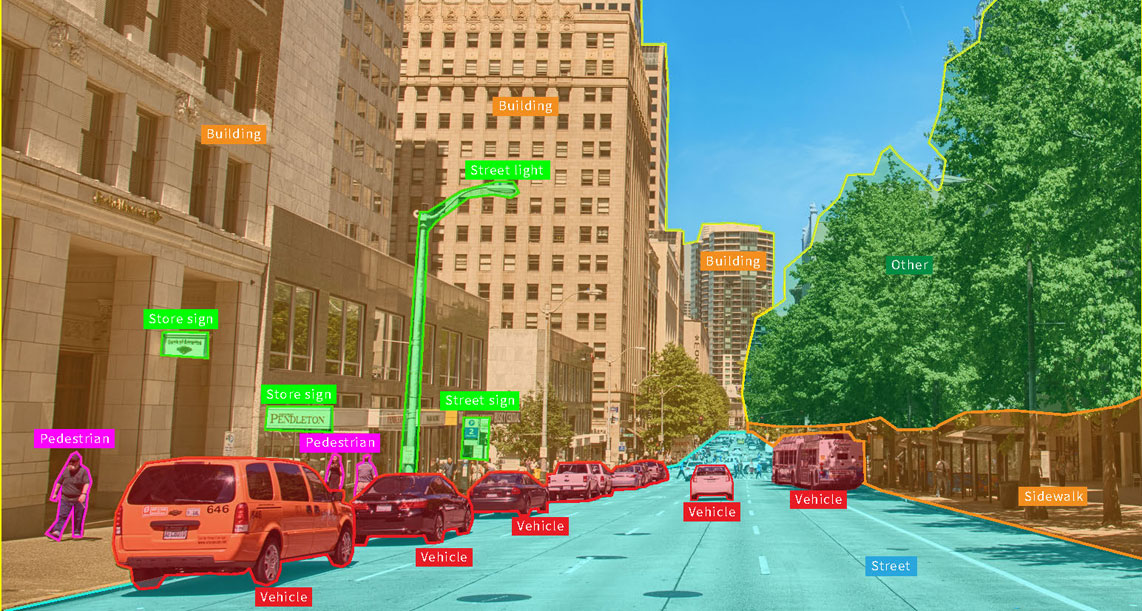
\includegraphics[keepaspectratio, scale=0.28]{pic/computer_vision.jpeg}
		\begin{tikzpicture}[remember picture,overlay]
			\node[anchor=south west, xshift=0.5cm, yshift=0.5cm] at (current page.south west) {
				\scriptsize Figure adapted from \href{https://www.linkedin.com/pulse/computer-vision-market-report-2022-27-size-share-demand-abhay-rajput}{source}
			};
		\end{tikzpicture}
		
	\end{frame}
	\begin{frame}{What Is Computer Vision?}
		\centering
		\begin{minipage}{0.4\textwidth}
			\centering
			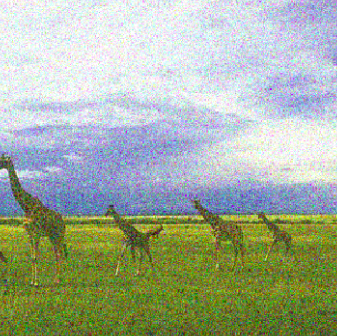
\includegraphics[width=\textwidth, keepaspectratio]{pic/noisy_image.png}
			\\Noisy image
		\end{minipage}%
		\hspace{0.1\textwidth} % Adjusts space between the two images
		\begin{minipage}{0.4\textwidth}
			\centering
			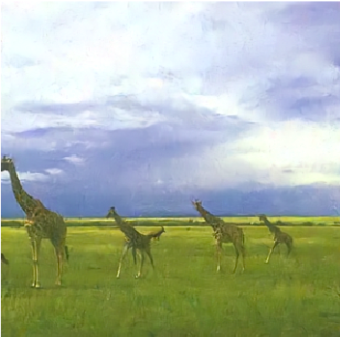
\includegraphics[width=\textwidth, keepaspectratio]{pic/denoised_image.png}
			\\Denoised image
		\end{minipage}
		\begin{tikzpicture}[remember picture,overlay]
			\node[anchor=south west, xshift=0.5cm, yshift=0.5cm] at (current page.south west) {
				\scriptsize Figure adapted from \href{https://github.com/lychengrex/Image-Denoising-with-Deep-CNNs/blob/master/src/tutorial.ipynb}{source}
			};
		\end{tikzpicture}
	\end{frame}
	\begin{frame}{What Is Computer Vision?}
		\centering
		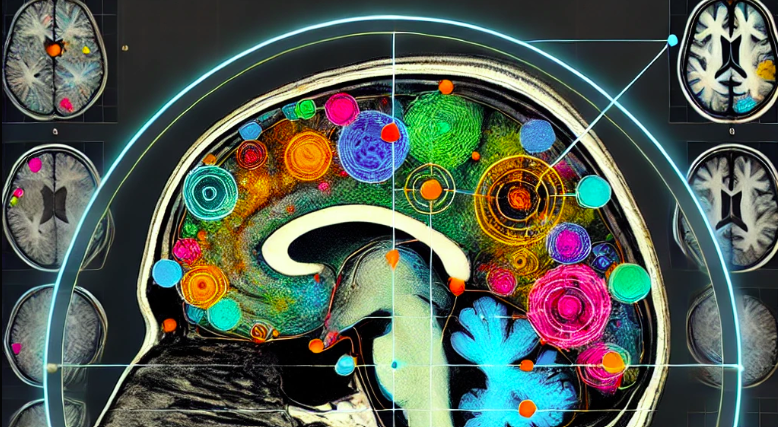
\includegraphics[keepaspectratio, scale=0.7]{pic/medical.png}
	\end{frame}
	\begin{frame}{Hand-crafted Features: Before Deep Learning Features}
		\begin{flushleft}
			\textbf{Two types} of features used for action recognition.
		\end{flushleft}
		
		\centering
		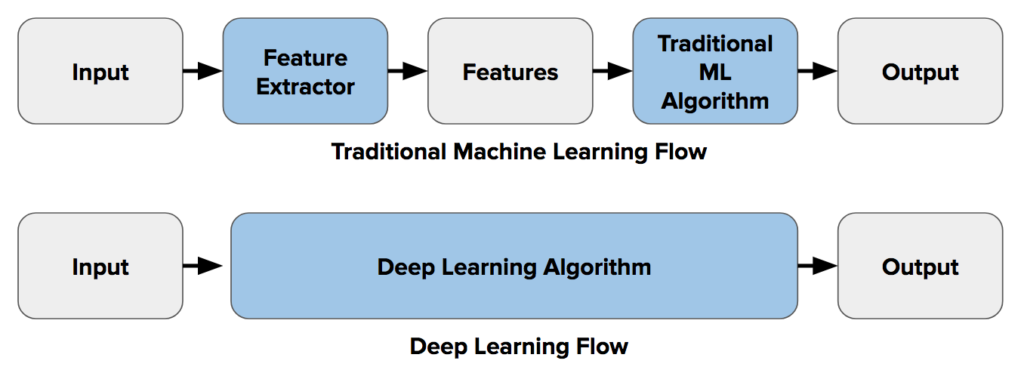
\includegraphics[keepaspectratio, scale=0.44]{pic/handcrafted_features.png}\\
		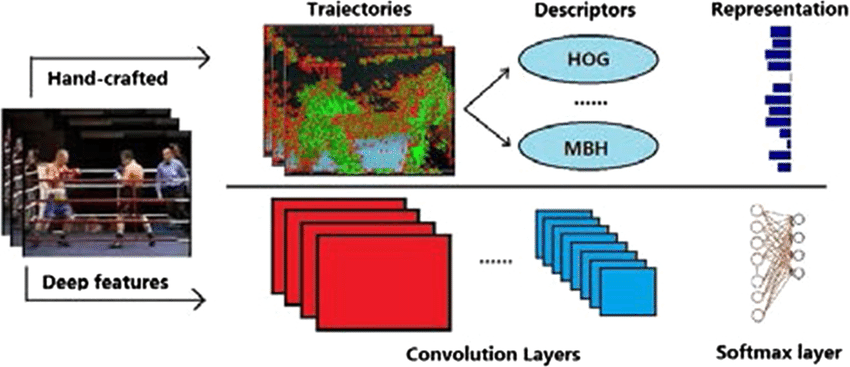
\includegraphics[keepaspectratio, scale=0.27]{pic/Two-types-of-features-used-for-action-recognition-ie-hand-crafted-features-and-deep.png}
		
		\begin{tikzpicture}[remember picture,overlay]
			\node[anchor=south west, xshift=0.5cm, yshift=0.5cm] at (current page.south west) {
				\scriptsize Figure adapted from \href{https://www.researchgate.net/figure/Two-types-of-features-used-for-action-recognition-ie-hand-crafted-features-and-deep_fig2_334897608}{source} \& \href{https://datascience.stackexchange.com/questions/54390/what-is-the-difference-between-handcrafted-and-learned-features}{source}
			};
		\end{tikzpicture}
		
	\end{frame}
	\begin{frame}{Hand-crafted Features: Before Deep Learning Features}
		\centering
		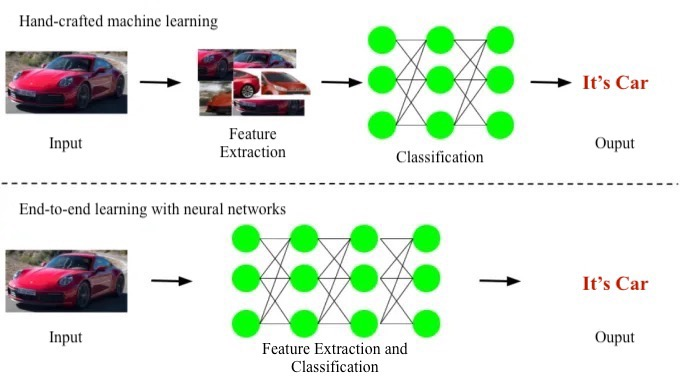
\includegraphics[keepaspectratio, scale=0.5]{pic/do-machine-learning-neural-networks-tasks-using-python copy 3.jpg}
		\begin{tikzpicture}[remember picture,overlay]
			\node[anchor=south west, xshift=0.5cm, yshift=0.5cm] at (current page.south west) {
				\scriptsize Figure adapted from \href{https://www.smlease.com/entries/technology/machine-learning-vs-deep-learning-what-is-the-difference-between-ml-and-dl/}{source}
			};
		\end{tikzpicture}
	\end{frame}
	\begin{frame}{Image Features}
		\begin{flushleft}
			
			\small{Fusion of multi-scale bag of deep visual words features of chest X-ray images to detect COVID-19 infection}
		\end{flushleft}
		\centering
		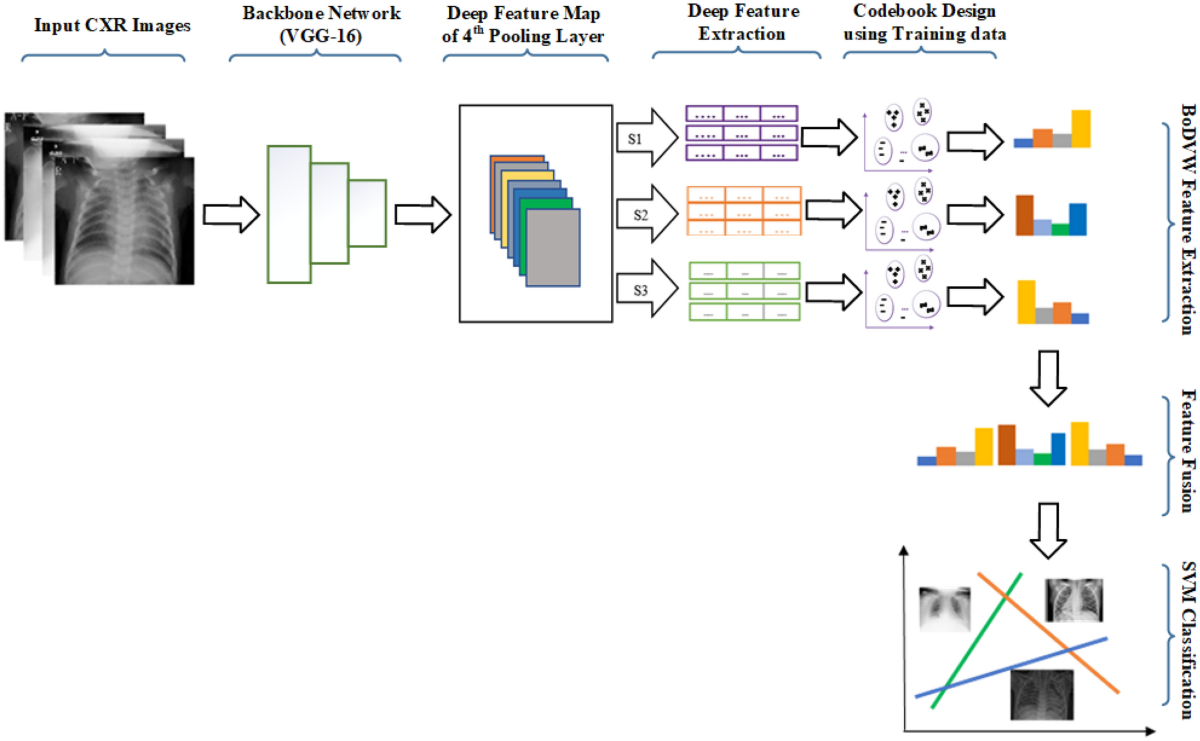
\includegraphics[keepaspectratio, scale=0.23]{pic/image_features.png}\\
		\begin{tikzpicture}[remember picture,overlay]
			\node[anchor=south west, xshift=0.5cm, yshift=0.5cm] at (current page.south west) {
				\scriptsize Figure adapted from \href{https://www.nature.com/articles/s41598-021-03287-8}{source}
			};
		\end{tikzpicture}
	\end{frame}
	\begin{frame}{Effect Of DL}
		\begin{flushleft}
			\small{Comparison between Deep Learning and Traditional Models}
		\end{flushleft}
		\centering
		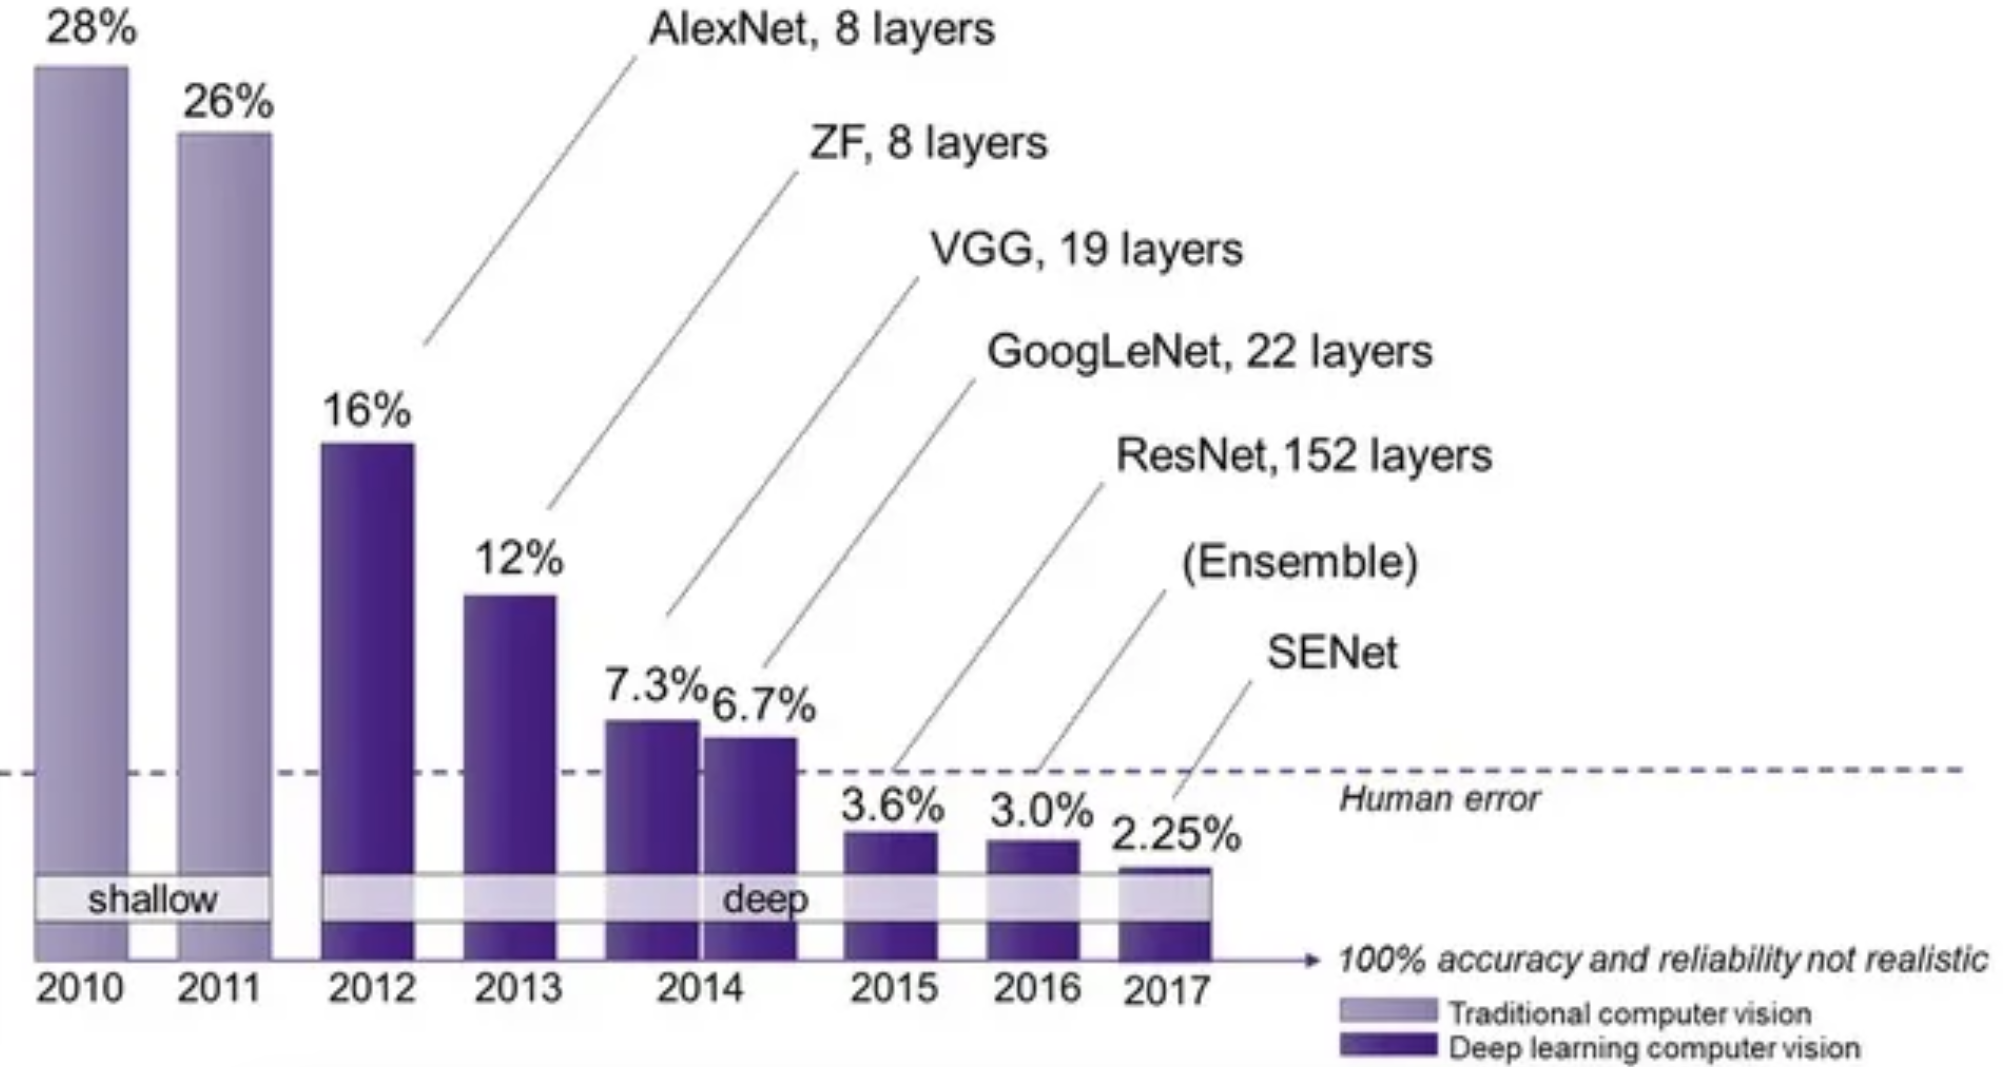
\includegraphics[keepaspectratio, scale=0.25]{pic/Synopsys_computer-vision-processors.png}
		\begin{tikzpicture}[remember picture,overlay]
			\node[anchor=south west, xshift=0.5cm, yshift=0.5cm] at (current page.south west) {
				\scriptsize Figure adapted from \href{https://dwbi1.wordpress.com/2021/07/01/what-is-convolution/}{source}
			};
		\end{tikzpicture}
	\end{frame}
	\section{CNN vs. FCN}
	\begin{frame}{FCNs On Images}
		\begin{itemize}
			\item What we've been using?
			\begin{itemize}
				\item \textbf{Dense} Vector Multiplication
			\end{itemize}
		\end{itemize}
		\begin{center}
			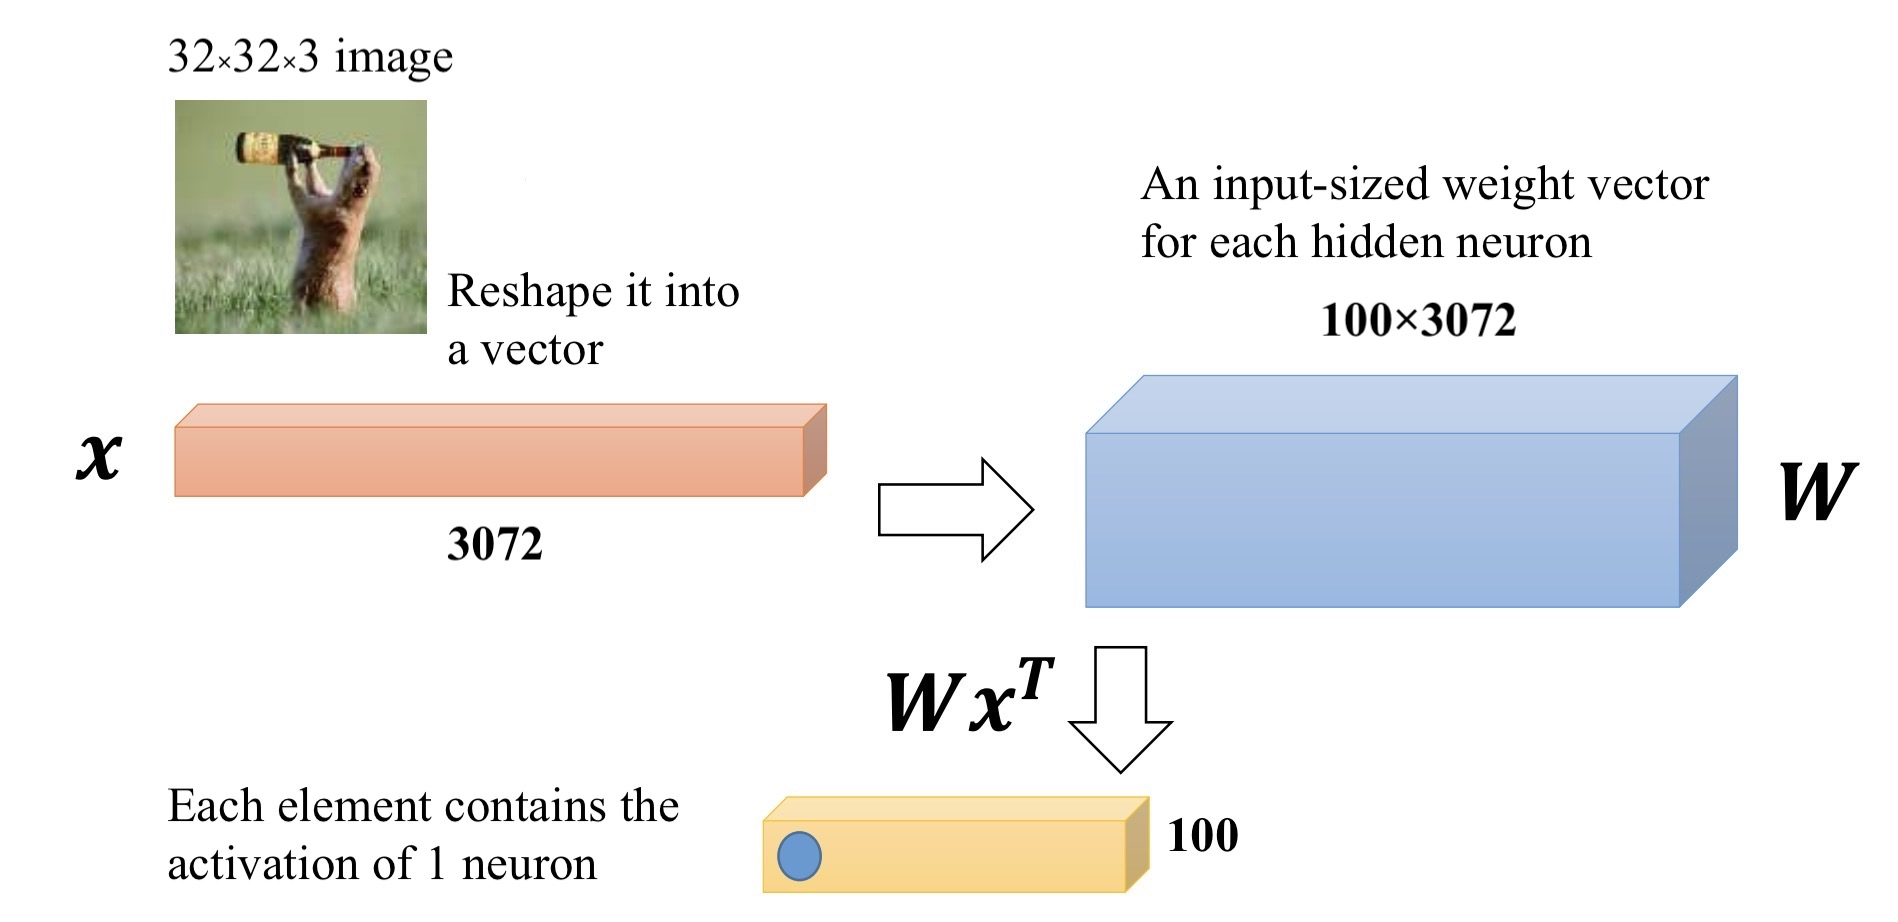
\includegraphics[keepaspectratio, scale=0.16]{pic/Processing images.jpg}
		\end{center}
		\vfill
		\begin{tikzpicture}[remember picture,overlay]
			\node[anchor=south west, xshift=0.5cm, yshift=0.5cm] at (current page.south west) {
				\scriptsize Figure adapted from [3]
			};
		\end{tikzpicture}
		
	\end{frame}
	\begin{frame}{Fully Connected Layers}
		\begin{itemize}
			\item Neurons in a single layer operate independently and \textbf{do not share connections}, even for inputs.
			
			\bigskip
			
			\item To be shift-invariant, \textbf{many samples} (in various time or locations) must be shown to them.
			
			\bigskip
			
			\item \textbf{Regular Neural Nets don’t scale well to full images}.
			\begin{itemize}
				\item Parameters would \textbf{add up} quickly!
				\item Full connectivity is wasteful and the huge number of parameters would quickly \textbf{lead to overfitting}.
			\end{itemize}
		\end{itemize}
	\end{frame}
	\begin{frame}{Solution?}
		\centering
		\large \textbf{What can we do?}
	\end{frame}
	\begin{frame}{Invariance VS. Equivariance}
		\begin{itemize}
			\item \textbf{Invariance:} \small The output \textbf{remains the same} when the input undergoes a transformation.
			\item \textbf{Equivariance:} \small The output \textbf{varies predictably} when the input undergoes a transformation.
			
		\end{itemize}
		\begin{center}
			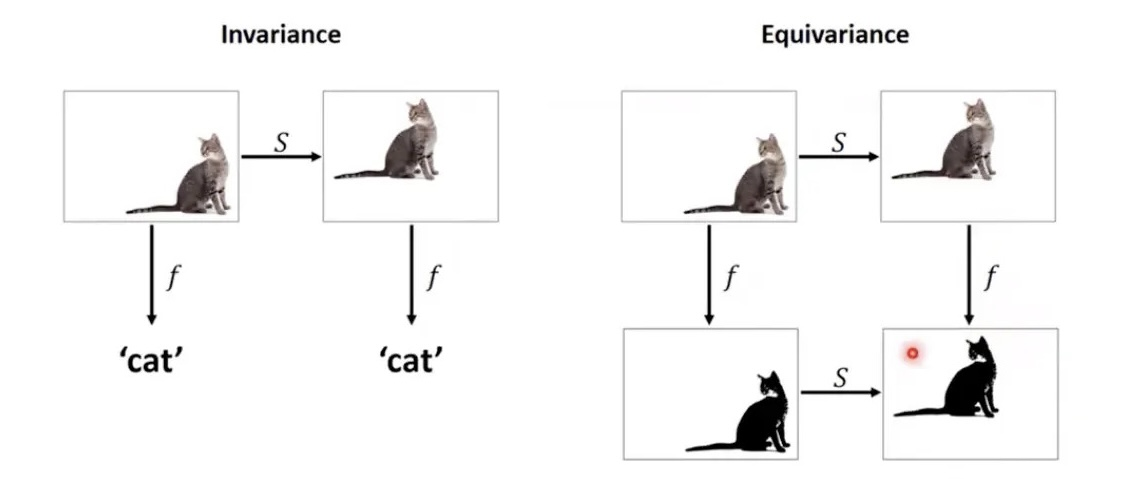
\includegraphics[keepaspectratio, scale=0.28]{pic/invariance_vs_equivariance.jpg}
		\end{center}
		\begin{tikzpicture}[remember picture,overlay]
			\node[anchor=south west, xshift=0.5cm, yshift=0.5cm] at (current page.south west) {
				\scriptsize Figure adapted from \href{https://medium.com/@sue.sk.guo/all-you-should-know-about-translation-equivariance-invariance-in-cnn-cbf2a2ad33cd}{source}
			};
		\end{tikzpicture}
		
	\end{frame}
	\begin{frame}{Shift-invariance}
		\begin{center}
			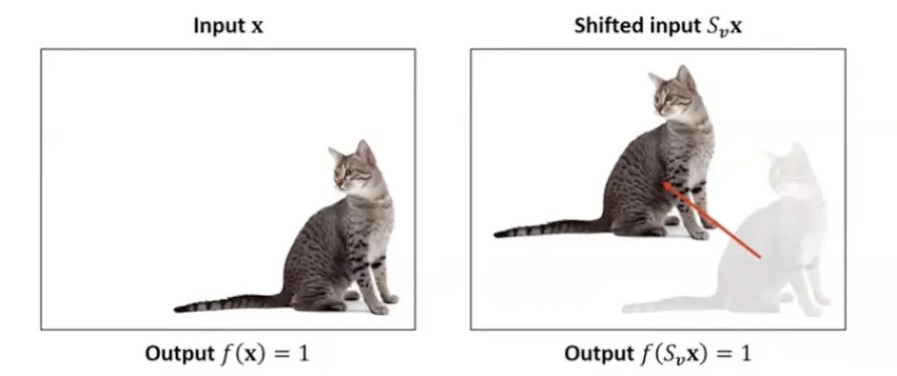
\includegraphics[keepaspectratio, scale=0.25]{pic/shift_invariance.jpg}
		\end{center}
		
		\begin{itemize}
			\item \textit{Cat detector} \quad $f: \mathbb{R}^d \to \mathbb{R}$
			
			\item \textit{Shift operator} \quad $S_v: \mathbb{R}^d \to \mathbb{R}^d$ \quad shifting the image by vector $v$
		\end{itemize}
		
		\textbf{Shift invariance:} \quad $f(\mathbf{x}) = f(S_v \mathbf{x})$
		\\ \textbf{Question: }{Will an MLP that recognizes the left image as a cat also recognize the shifted image on the right as a cat?}
	\end{frame}
	\begin{frame}{A Problem}
		\begin{itemize}
			\item In many problems the \textbf{location} of a pattern is not important.
			\begin{itemize}
				\item Only the \textbf{presence} of the pattern matters.
			\end{itemize}
			\item Traditional MLPs are \textbf{sensitive} to pattern location.
			\begin{itemize}
				\item Moving it by one component results in an entirely different input that the MLP won’t recognize.
			\end{itemize}
			
			\item \textbf{Requirement:} Network must be \textbf{shift invariant}.
		\end{itemize}
	\end{frame}
	\begin{frame}{Convolution On Images}
		Convolution (Refresher)
		\begin{center}
			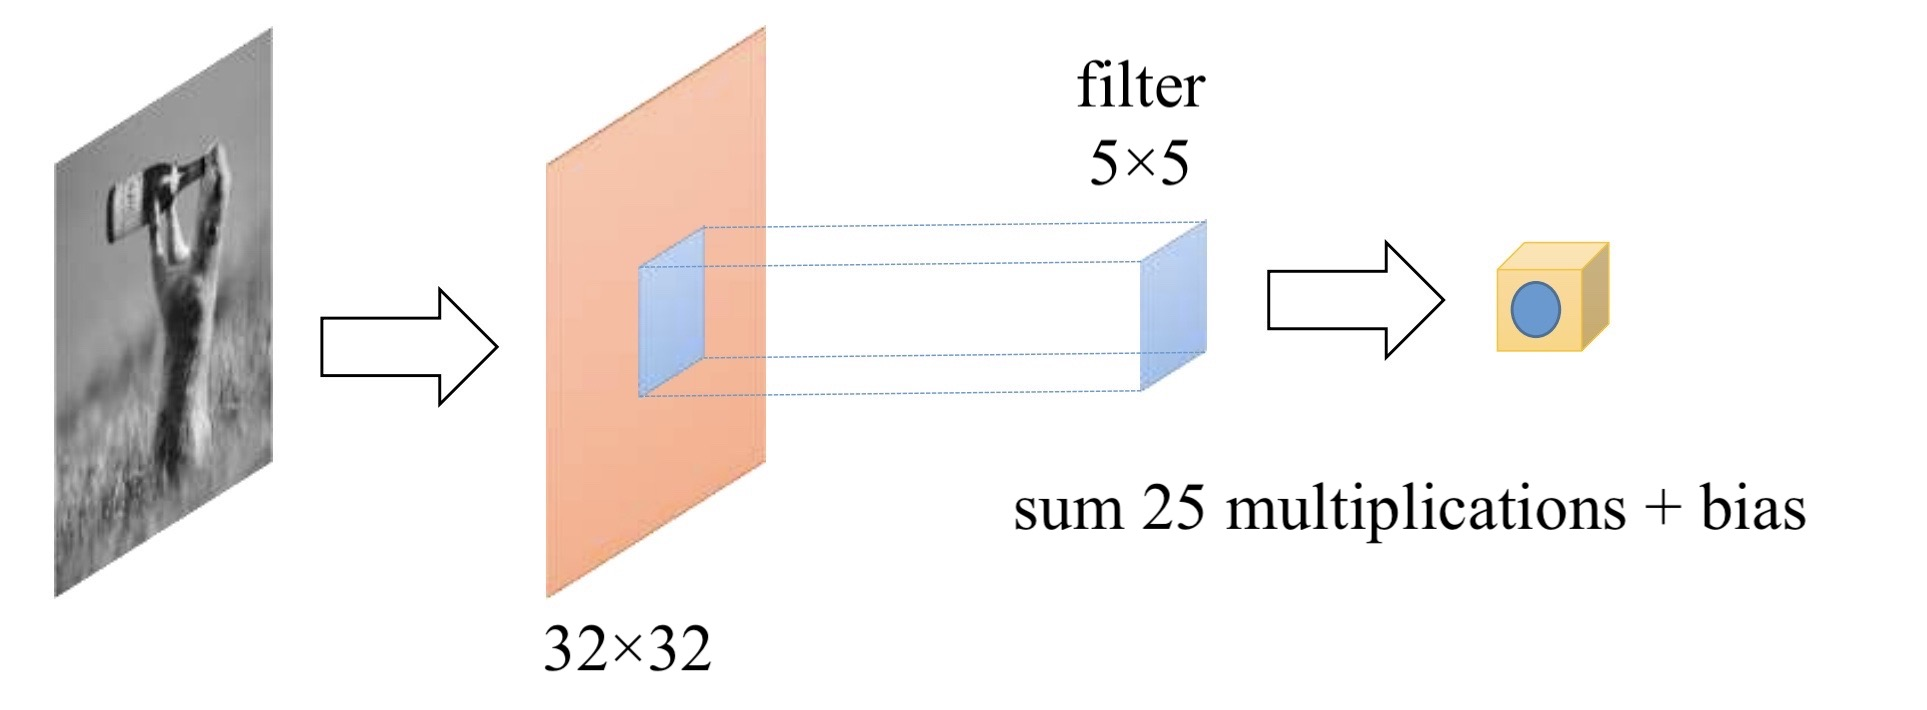
\includegraphics[keepaspectratio, scale=0.16]{pic/conv.jpg}
			
			
			Matrix input preserving \textbf{spatial structure}
			
			\vfill
			\begin{tikzpicture}[remember picture,overlay]
				\node[anchor=south west, xshift=0.5cm, yshift=0.5cm] at (current page.south west) {
					\scriptsize Figure adapted from [3]
				};
			\end{tikzpicture}
			
		\end{center}
		
	\end{frame}
	\begin{frame}{Fully Connected Or Convolution}
		
		\textbf{Question:}
		Can I just do classification on an flatten image (e.g., a 1080x1080x3 image) with fully connected layers?
		
		
	\end{frame}
	\begin{frame}{Fully Connected Or Convolution}
		
		\textbf{Question:}
		Can I just do classification on an flatten image (e.g., a 1080x1080x3 image) with fully connected layers?
		
		\bigskip
		
		\textbf{Answer:}
		No, using fully connected layers on such a large image is inefficient due to:
		\begin{itemize}
			\item Loss of spatial structure
			\item High parameter count
		\end{itemize}
		
		
	\end{frame}
	
	\begin{frame}{Fully Connected Or Convolution}
		
		\textbf{Why Use Convolution:}
		\begin{itemize}
			\item \textbf{Exploit spatial structure:} Convolution sees local patterns by using filters over small patches of the image.
			\item \textbf{Reduce parameters:} By sharing weights across the image, convolution reduce the number of parameters.
			\item \textbf{Build hierarchical features:} Convolution starts with small patterns, then combines them to recognize more complex patters.
		\end{itemize}
		
	\end{frame}
	\begin{frame}
		\centering
		% Left column with one centered image
		\begin{minipage}{0.5\textwidth}
			\centering
			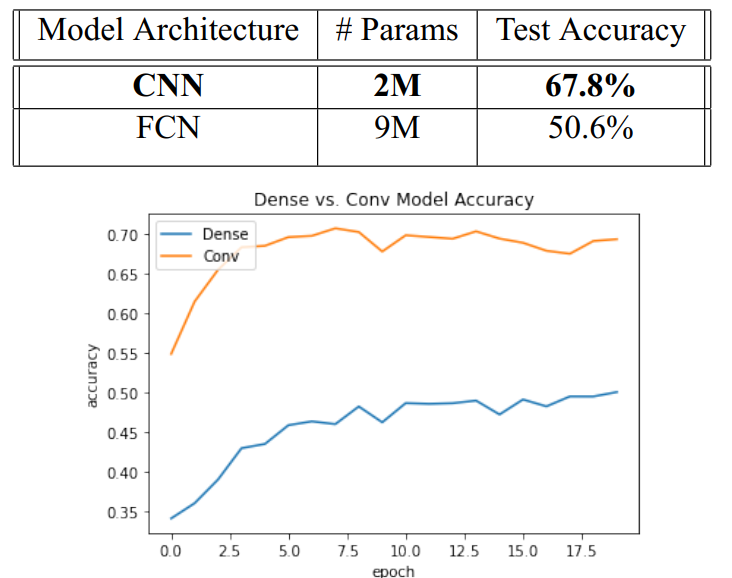
\includegraphics[keepaspectratio, scale=0.55]{pic/param.png}
		\end{minipage}
		\hfill
		% Right column with two images stacked on top of each other
		\begin{minipage}{0.4\textwidth}
			\centering
			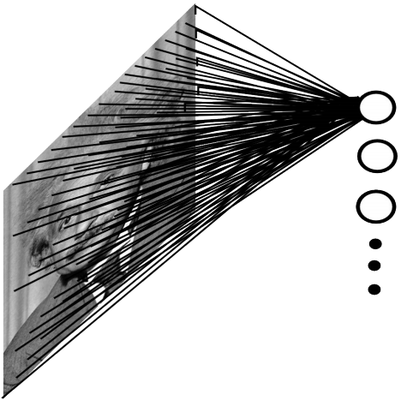
\includegraphics[keepaspectratio, scale=0.4]{pic/FCN.png} \\
			\vspace{0.3cm} % Space between the two images on the right
			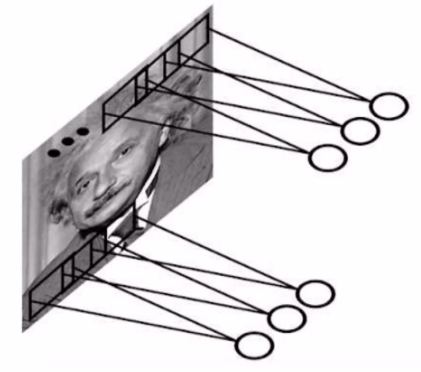
\includegraphics[keepaspectratio, scale=0.4]{pic/CNn.png}
		\end{minipage}
		
		\vfill
		\begin{tikzpicture}[remember picture,overlay]
			\node[anchor=south west, xshift=0.5cm, yshift=0.5cm] at (current page.south west) {
				\scriptsize Figure adapted from \href{https://www.researchgate.net/figure/A-Typical-Architecture-of-CNNs-by-Tajbakhsh-2016_fig1_367165856}{source}
			};
		\end{tikzpicture}
	\end{frame}
	
	\begin{frame}{What Is CNN?}
		\begin{itemize}
			\item It is a class of deep learning.
			
			\item Convolutional neural network (ConvNet’s or CNNs) is one of the main categories to do image recognition, image classifications, object detection, recognition of faces, etc.
			
			\item It is \textbf{similar to the basic neural network}. CNNs also have learnable parameters like weights and biases, similar to neural networks.
			
			\item CNN is heavily used in \textbf{computer vision}.
			
			\item There are \textbf{3 basic components} to define CNN:
			\begin{itemize}
				\item The Convolution Layer
				\item The Pooling Layer
				\item The Output Layer or Fully Connected Layer
			\end{itemize}
		\end{itemize}
		
	\end{frame}
	\begin{frame}{Architecture Of CNN}
		\centering
		The basic idea of Convolutional Neural Networks (CNNs) is similar to Backpropagation Neural Networks (BPNNs) but differs in implementation.
		
		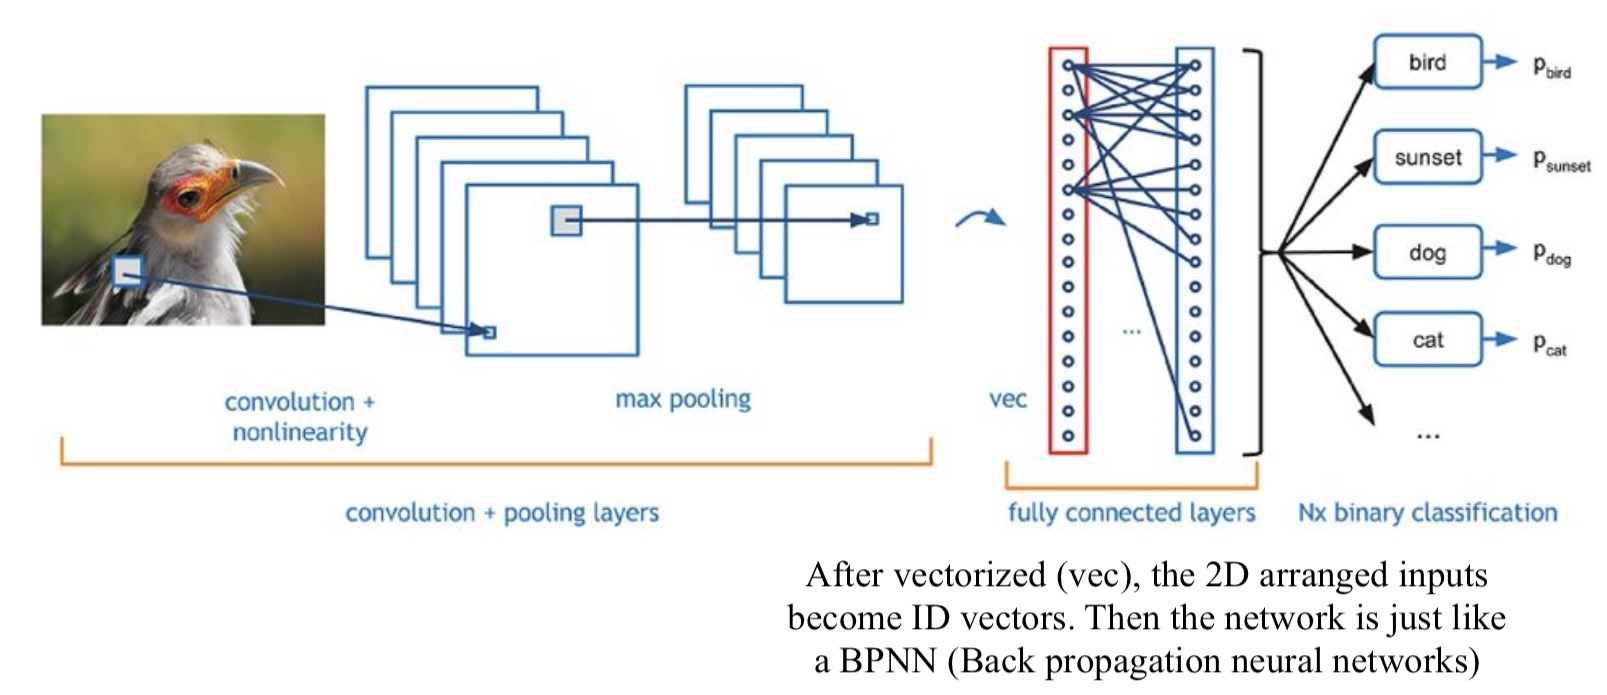
\includegraphics[keepaspectratio, scale=0.5]{pic/Architecture_of_CNN.jpg}
		
		\vfill
		\begin{tikzpicture}[remember picture,overlay]
			\node[anchor=south west, xshift=0.5cm, yshift=0.5cm] at (current page.south west) {
				\scriptsize Figure adapted from \href{https://www.researchgate.net/figure/A-Typical-Architecture-of-CNNs-by-Tajbakhsh-2016_fig1_367165856}{source}
			};
		\end{tikzpicture}
	\end{frame}
	\begin{frame}{The Basic Structure}
		\begin{itemize}
			\item Alternating \textbf{Convolution (C)} and \textbf{subsampling layer (S)}
			\item Subsampling allows flexible positioning of features.
		\end{itemize}
		\begin{center}
			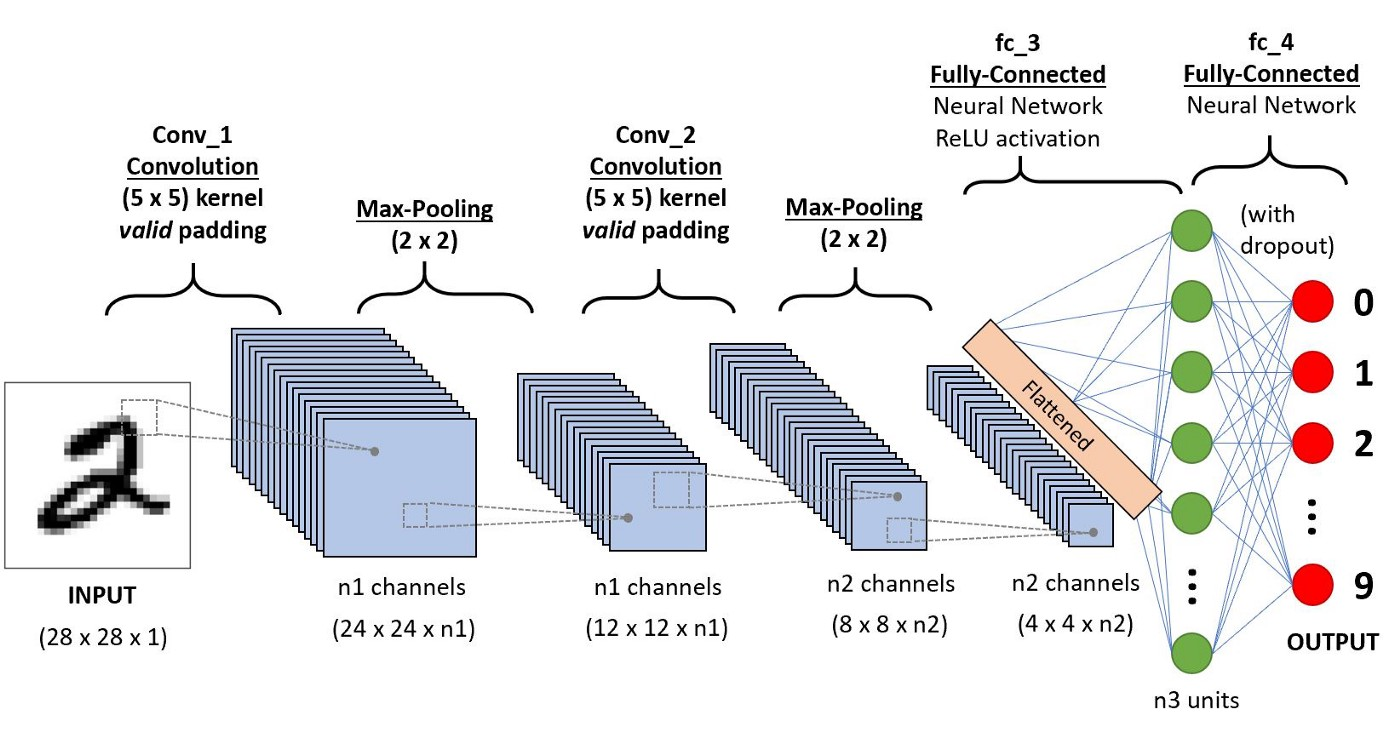
\includegraphics[keepaspectratio, scale=0.2]{pic/CNN_structure_a.jpeg}
		\end{center}
		\vfill
		\begin{tikzpicture}[remember picture,overlay]
			\node[anchor=south west, xshift=0.5cm, yshift=0.5cm] at (current page.south west) {
				\scriptsize Figure adapted from \href{https://www.plainconcepts.com/convolutional-neural-network-guide/}{source}
			};
		\end{tikzpicture}
	\end{frame}
	
	\begin{frame}{The Basic Structure}
		\item \textbf{Three Main Types of Layers}
		\begin{itemize}
			\item \textbf{Convolutional Layer}
			\begin{itemize}
				\item Output of neurons are connected to \textbf{local regions} in the input.
				\item Applying the \textbf{same filter} across the entire image.
				\item CONV layer’s parameters consist of a set of \textbf{learnable filters}.
			\end{itemize}
			\item \textbf{Pooling Layer}
			\begin{itemize}
				\item Performs a \textbf{downsampling} operation along the spatial dimensions.
			\end{itemize}
			\item \textbf{Fully-Connected Layer}
			\begin{itemize}
				\item Typically used in the final stages of the network to combine high-level features and \textbf{make predictions}.
			\end{itemize}
		\end{itemize}
	\end{frame}
	\begin{frame}{CNN VS. FCN}
		\begin{itemize}
			\item \textbf{Fully Connected Networks (FCNs):}
			\begin{itemize}
				\item High number of parameters, leading to \textbf{overfitting on large inputs} (e.g., images).
				\item Lack of spatial awareness, making it \textbf{sensitive to the exact positioning} of patterns.
				\item Suitable for structured data but \textbf{inefficient for image processing}.
				
			\end{itemize}
			
			\item \textbf{Convolutional Neural Networks (CNN):}
			\begin{itemize}
				\item Uses filters to process only small parts of the input at a time (\textbf{locality}).
				\item Weight sharing and local connectivity \textbf{reduce the number of parameters}.
				\item Can recognize patterns independent of their location within the image (\textbf{shift invariance}).
				\item \textbf{Efficient} for image, video, and speech data.
			\end{itemize}
			
		\end{itemize}
	\end{frame}
	
	 \section{Convolution}
	\begin{frame}{What Is A Convolve}
		\centering
		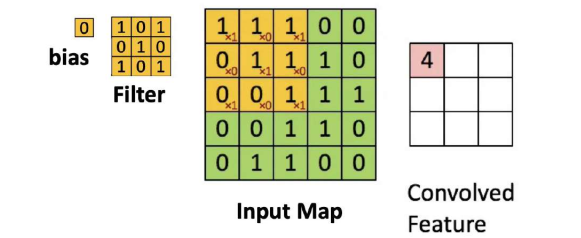
\includegraphics[keepaspectratio, scale=0.9]{pic/convo.png}
		\\
		\textbf{Scanning an image with a "filter"}
		
		\begin{itemize}
			\item A filter is really \textbf{just a perceptron}, with weights and a bias.
			\item At each location, the filter is\textbf{ multiplied component-wise} with the underlying map values, and the products are summed along with the bias.
		\end{itemize}
		\vfill
		\begin{tikzpicture}[remember picture,overlay]
			\node[anchor=south west, xshift=0.5cm, yshift=0.5cm] at (current page.south west) {
				\scriptsize Figure adapted from [3]
			};
		\end{tikzpicture}
		
	\end{frame}
	\begin{frame}{Weights Showing Correlation}
		\centering
		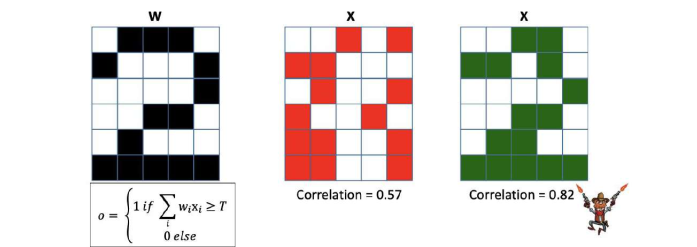
\includegraphics[keepaspectratio, scale=0.9]{pic/corr.png}
		\definecolor{darkgreen}{rgb}{0.0, 0.5, 0.0}
		\begin{itemize}
			\item The \textbf{weights} of the filter \textbf{represent the appearance} of the number "2".
			\item The \textcolor{deepgreen}{green} has a higher correlation with the filter compared to the \textcolor{red}{red}.
			\item The \textcolor{deepgreen}{green pattern} is more likely to represent the number "2".
		\end{itemize}
		
		\vfill
		\begin{tikzpicture}[remember picture,overlay]
			\node[anchor=south west, xshift=0.5cm, yshift=0.5cm] at (current page.south west) {
				\scriptsize Figure adapted from [1]
			};
		\end{tikzpicture}
	\end{frame}
	\begin{frame}{What Is Convolution}
		\centering
		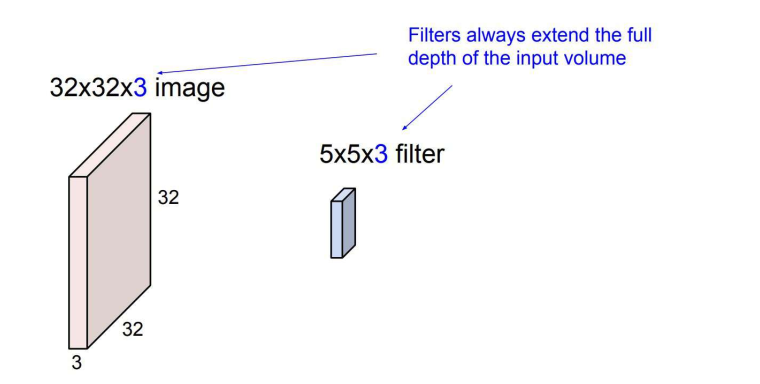
\includegraphics[keepaspectratio, scale=0.5]{pic/img.png}
		
		\smallskip
		\begin{itemize}
			\item \textbf {Convolve:} Slide over the image spatially, computing dot products.
			\item This allows us to \textbf{preserve the spatial structure} of the input.
		\end{itemize}
		
		\vfill
		\begin{tikzpicture}[remember picture,overlay]
			\node[anchor=south west, xshift=0.5cm, yshift=0.5cm] at (current page.south west) {
				\scriptsize Figure adapted from [2]
			};
		\end{tikzpicture}
		
	\end{frame}
	\begin{frame}{What Is The Output}
		\centering
		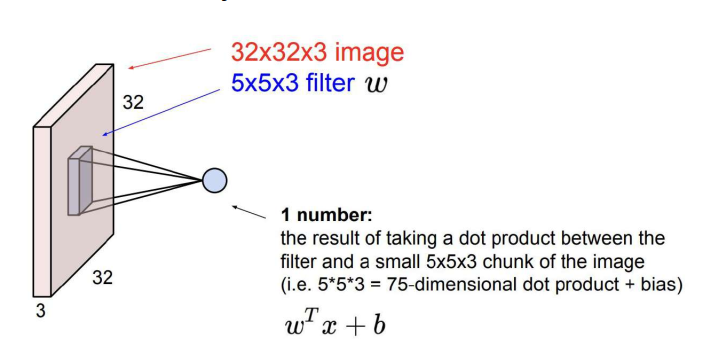
\includegraphics[keepaspectratio, scale=0.8]{pic/img1.png}
		\begin{itemize}
			\item It's simply a neuron with local connectivity!
		\end{itemize}
		
		\vfill
		\begin{tikzpicture}[remember picture,overlay]
			\node[anchor=south west, xshift=0.5cm, yshift=0.5cm] at (current page.south west) {
				\scriptsize Figure adapted from [2]
			};
		\end{tikzpicture}
	\end{frame}
	
	\frame{\frametitle{Convolution Process}
		\begin{itemize}
			\item \normalsize Consider this as the filter we are going to use:
		\end{itemize}
		\begin{figure}
			\centering
			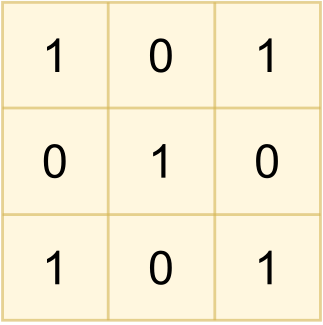
\includegraphics[keepaspectratio, scale=0.4]{pic/kernel5.png}
		\end{figure}
	}
	\begin{frame}{Convolution Process}
		\begin{itemize}
			\item \normalsize This is how we calculate the convolutional layer's output:
		\end{itemize}
		\small
		\begin{equation*}
			\text{Convolved Feature}(i, j) = (I * K)(i, j) = \sum_{a=0}^{k_h - 1} \sum_{b=0}^{k_w - 1} I(i+a, j+b) K(a, b)
		\end{equation*}
		I: Input Image\newline
		K: Our Kernel\newline
		$k_h$ and $k_w$: The height and width of the Kernel
		
	\end{frame}
	
	\foreach \i in {0,...,8}
	{
		\frame{\frametitle{Convolution Process}
			\begin{figure}
				\begin{itemize}
					\item \small Convoluting a 5x5x1 image with a 3x3x1 kernel to get a 3x3x1 convolved feature.
					
				\end{itemize}
				
				\centering
				\begin{minipage}{.1\textwidth}
					\centering
					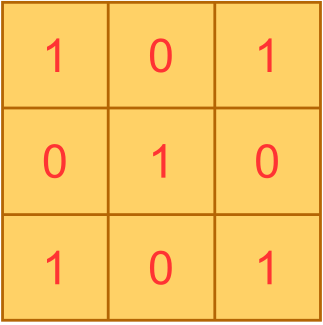
\includegraphics[keepaspectratio, scale=0.2]{pic/kernel6-1.png}
				\end{minipage}%
				\begin{minipage}{.9\textwidth}
					\centering
					\includegraphics[keepaspectratio, scale=0.45]{pic/kernel-frame-\i.png}
				\end{minipage}
				\vfill
				\begin{tikzpicture}[remember picture,overlay]
					\node[anchor=south west, xshift=0.5cm, yshift=0.5cm] at (current page.south west) {
						\scriptsize Figure adapted from [3]
					};
				\end{tikzpicture}
			\end{figure}
		}
	}
	
	\begin{frame}{To Summarize}
		\normalsize
		\begin{itemize}
			\item We apply the same filter on different regions of the input.
			\item Convolutional filters learn to make \textbf{decisions based on local spatial input}, which is an important attribute when working with images.
			\item Uses a lot \textbf{fewer parameters} compared to Fully Connected Layers.
		\end{itemize}
		\begin{figure}
			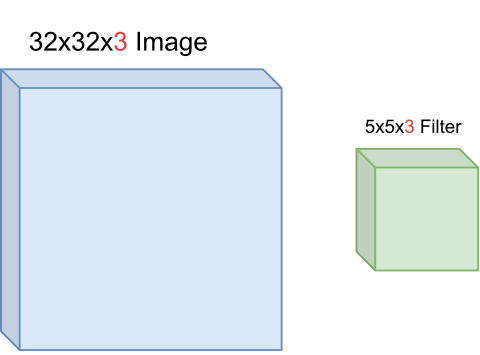
\includegraphics[keepaspectratio, scale=0.25]{pic/CNN2.png}
			\hspace{3cm}  % Adjust the distance as needed
			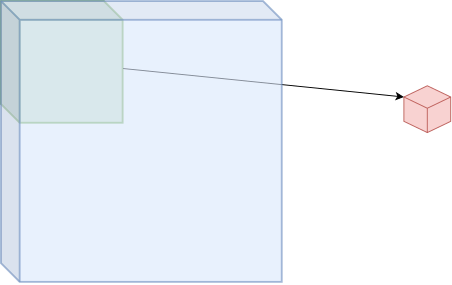
\includegraphics[keepaspectratio, scale=0.25]{pic/kernel2.png}
		\end{figure}
		
	\end{frame}
	
	\begin{frame}{Convolution Outlook}
		\centering
		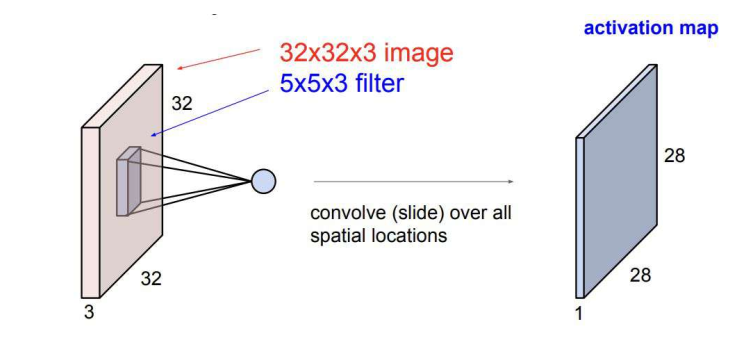
\includegraphics[keepaspectratio, scale=0.7]{pic/img5.png}
		\smallskip
		\begin{itemize}
			\item \small If we consider the \textbf{image} to be of size \textcolor{blue}{\( n \times m \times b \)} and the \textbf{filter} to be of size \textcolor{blue}{\( n' \times m' \times b \)}, we will have an \textbf{activation map} of size \textcolor{blue}{\( (n - n' + 1) \times (m - m' + 1) \times 1 \)} for each filter.
		\end{itemize}
		
		\vfill
		\begin{tikzpicture}[remember picture,overlay]
			\node[anchor=south west, xshift=0.5cm, yshift=0.5cm] at (current page.south west) {
				\scriptsize Figure adapted from [2]
			};
		\end{tikzpicture}
		
	\end{frame}
	\begin{frame}{Convolution Outlook}
		\centering
		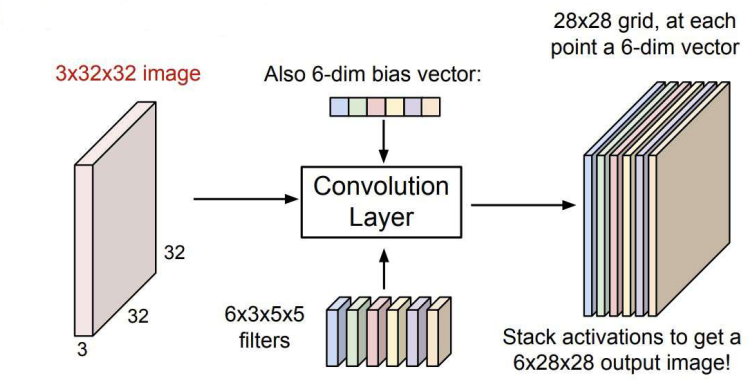
\includegraphics[keepaspectratio, scale=0.7]{pic/img6.png}
		\smallskip
		\begin{itemize}
			\item \small Multiple filters can be applied, each with its own bias, to extract different features from the input.
		\end{itemize}
		
		
		\vfill
		\begin{tikzpicture}[remember picture,overlay]
			\node[anchor=south west, xshift=0.5cm, yshift=0.5cm] at (current page.south west) {
				\scriptsize Figure adapted from [2]
			};
		\end{tikzpicture}
		
	\end{frame}
	
	\begin{frame}{What Is Stride}
		\centering
		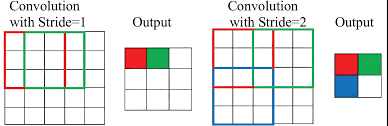
\includegraphics[keepaspectratio, scale=0.9]{pic/stride.png}
		\begin{itemize}
			\item The scans of the individual filters may \textbf{advance by more than one} pixel at a time.
			\begin{itemize}
				\item The \textbf{stride} can be greater than 1.
				\item Effectively increasing the granularity of the scan.
				\begin{itemize}
					\item \textbf{Saves computation}, sometimes at the risk of \textbf{losing information}.
				\end{itemize}
			\end{itemize}
			\item This results in a \textbf{reduction} in the size of the \textbf{resulting maps}.
			\begin{itemize}
				\item They will shrink by a factor equal to the stride.
			\end{itemize}
			\item This can happen at \textbf{any layer}.
		\end{itemize}
		
		
		\vfill
		\begin{tikzpicture}[remember picture,overlay]
			\node[anchor=south west, xshift=0.5cm, yshift=0.5cm] at (current page.south west) {
				\scriptsize Figure adapted from [3]
			};
		\end{tikzpicture}
	\end{frame}
	
	
	\begin{frame}{Stride-1}
		\vspace{0.5cm}
		
		\normalsize \textbf{Closer look}
		\begin{itemize}
			\item 7x7 input with 3x3 filter
			\item This was a Stride 1 filter
			\item=> Outputs 5x5
		\end{itemize}
		
		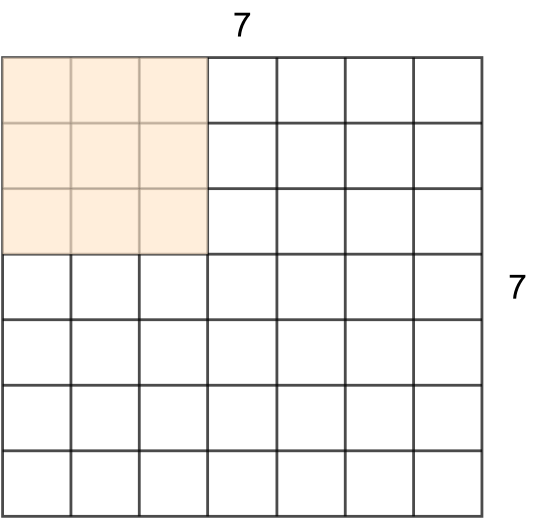
\includegraphics[keepaspectratio, scale=0.13]{pic/Stride1.png}
		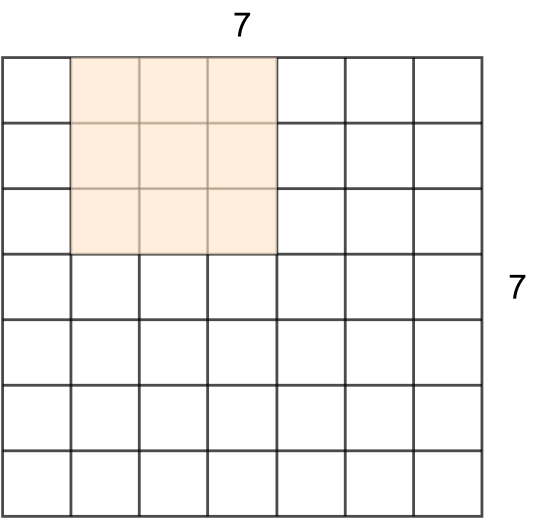
\includegraphics[keepaspectratio, scale=0.13]{pic/Stride2.png}
		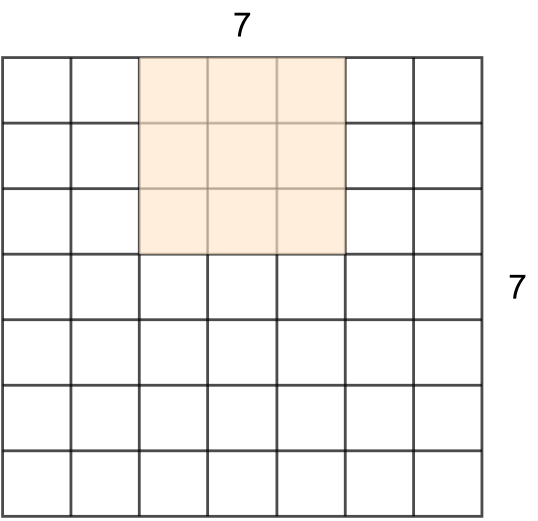
\includegraphics[keepaspectratio, scale=0.13]{pic/Stride3.png}
		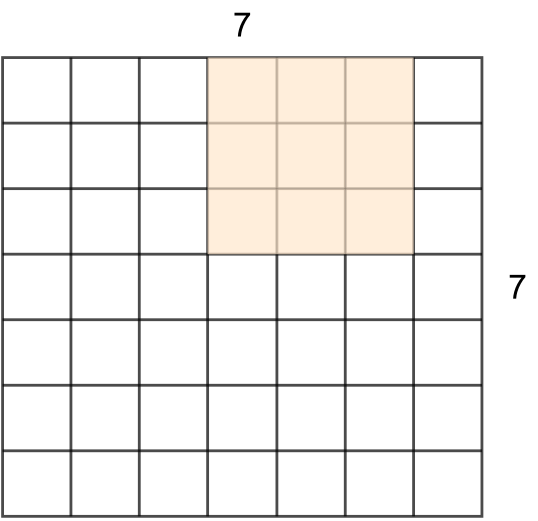
\includegraphics[keepaspectratio, scale=0.13]{pic/Stride4.png}
		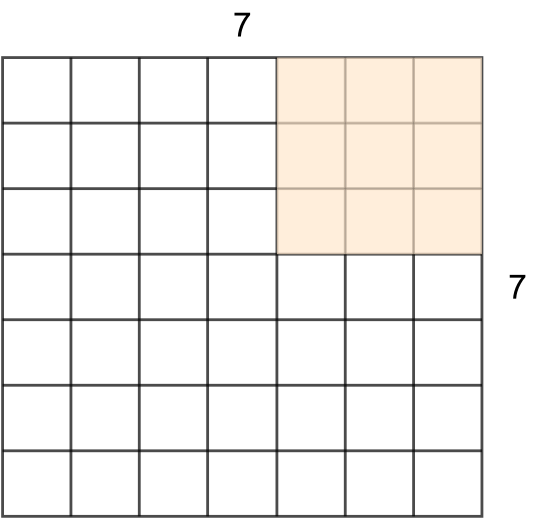
\includegraphics[keepaspectratio, scale=0.13]{pic/Stride5.png}
		
	\end{frame}
	
	
	
	
	
	\begin{frame}{Strides-2}
		\vspace{0.5cm}
		
		\normalsize Now let's use Stride 2
		\begin{itemize}
			\item 7x7 input with 3x3 filter
			\item This was a Stride 2 filter
			\item=> Outputs 3x3
		\end{itemize}
		
		\centering
		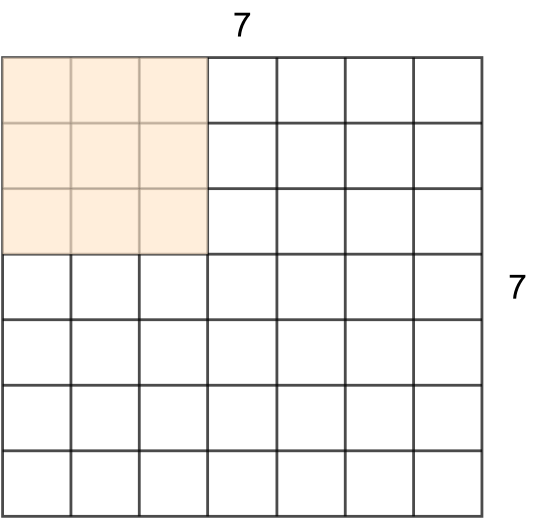
\includegraphics[keepaspectratio, scale=0.2]{pic/Stride6.png}
		\hspace{0.2cm}
		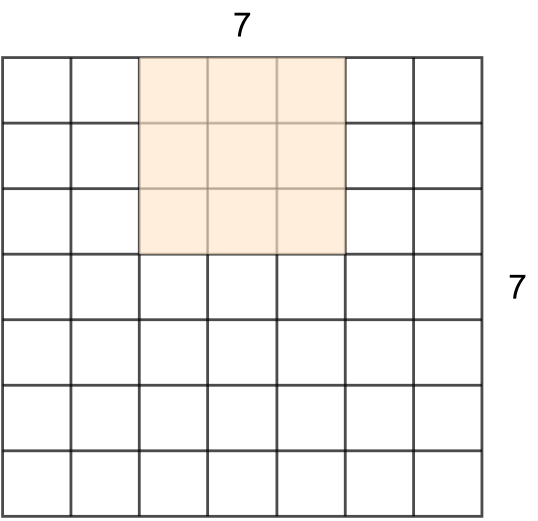
\includegraphics[keepaspectratio, scale=0.2]{pic/Stride7.png}
		\hspace{0.2cm}
		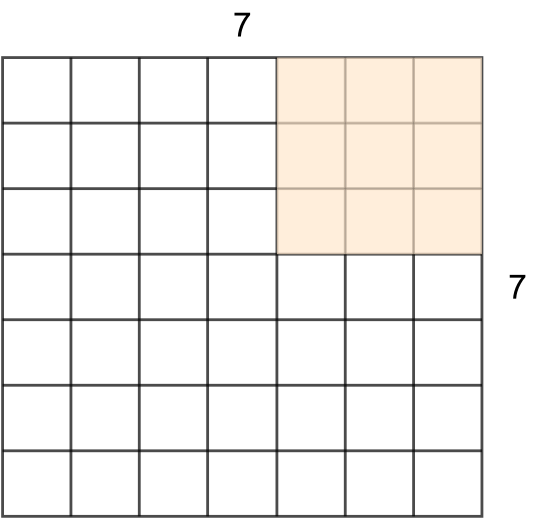
\includegraphics[keepaspectratio, scale=0.2]{pic/Stride8.png}
		
	\end{frame}
	\begin{frame}{Strides-3}
		\vspace{0.5cm}
		
		\textbf{What about Stride 3?}
		\begin{itemize}
			\item 7x7 input with 3x3 filter
		\end{itemize}
		
		\centering
		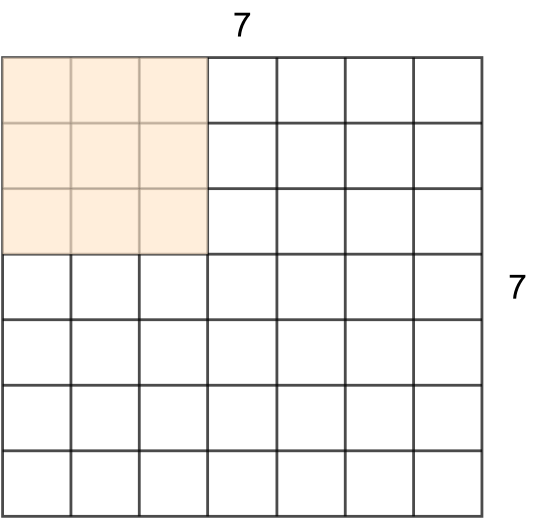
\includegraphics[keepaspectratio, scale=0.2]{pic/Stride9.png}
		\hspace{0.2cm}
		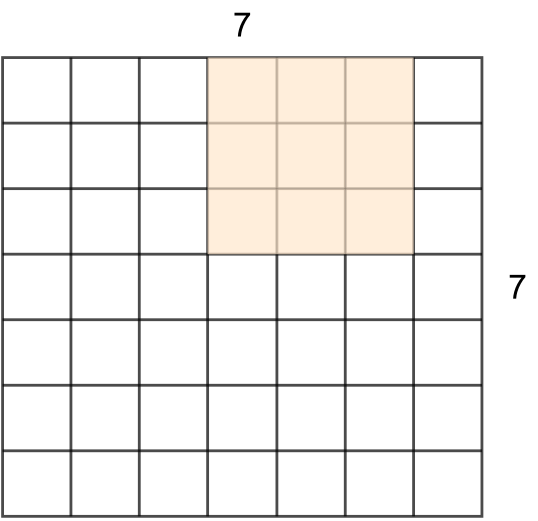
\includegraphics[keepaspectratio, scale=0.2]{pic/Stride10.png}
		\hspace{0.2cm}
		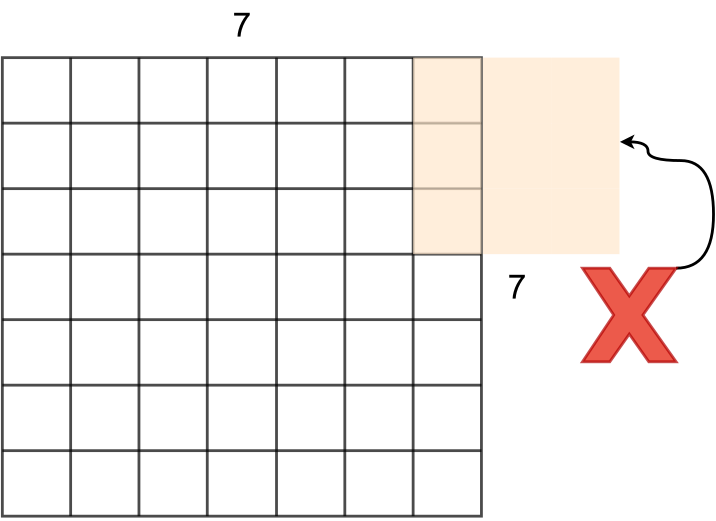
\includegraphics[keepaspectratio, scale=0.2]{pic/Stride11.png}
		
		
	\end{frame}
	\begin{frame}{Strides Formula}
		
		\begin{minipage}{0.4\textwidth}
			\centering
			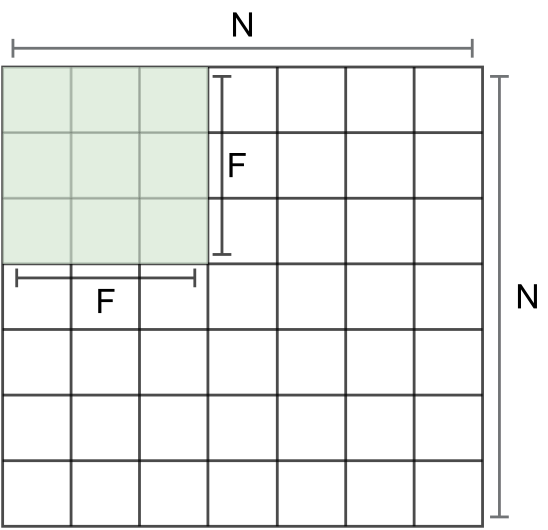
\includegraphics[keepaspectratio, scale=0.25]{pic/Stride12.png}
		\end{minipage}%
		\hspace{0.5cm}  % Adjust spacing between image and text
		\begin{minipage}{0.55\textwidth}
			\textbf{\large $Output Size = \frac{(N - F)}{\text{Stride}} + 1$}
			
			\vspace{0.3cm}
			
			\( N = 7, F = 3 \Rightarrow \)
			\begin{itemize}
				\item Stride 1: \( (7 - 3) / 1 + 1 = 5 \)
				\item Stride 2: \( (7 - 3) / 2 + 1 = 3 \)
				\item \textbf{Stride 3: \( (7 - 3) / 3 + 1 = 2.33 \) !!!}
			\end{itemize}
		\end{minipage}
		
		\vfill
		\begin{tikzpicture}[remember picture,overlay]
			\node[anchor=south west, xshift=0.5cm, yshift=0.5cm] at (current page.south west) {
				\scriptsize Figure adapted from [2]
			};
		\end{tikzpicture}
		
	\end{frame}
	\begin{frame}{A problem?}
		\begin{center}
			\LARGE What could cause problems?
		\end{center}
	\end{frame}
	\begin{frame}{Problem-1}
		
		\begin{itemize}
			\item \Large \textbf{The borders don't get enough attention.}
			\item \Large Outputs shrink!
		\end{itemize}
		
		\centering
		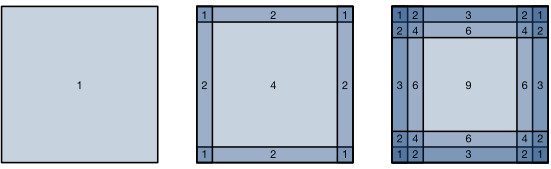
\includegraphics[keepaspectratio, scale=0.4]{pic/padding1.png}
		
		\small Pixel utilization for convolutions of size $1 \times 1$, $2 \times 2$, and $3 \times 3$ respectively.
	\end{frame}
	\begin{frame}{Problem-2}
		
		\begin{itemize}
			\item \Large Borders don't get enough attention.
			\item \Large \textbf{Outputs shrink!}
		\end{itemize}
		
		\centering
		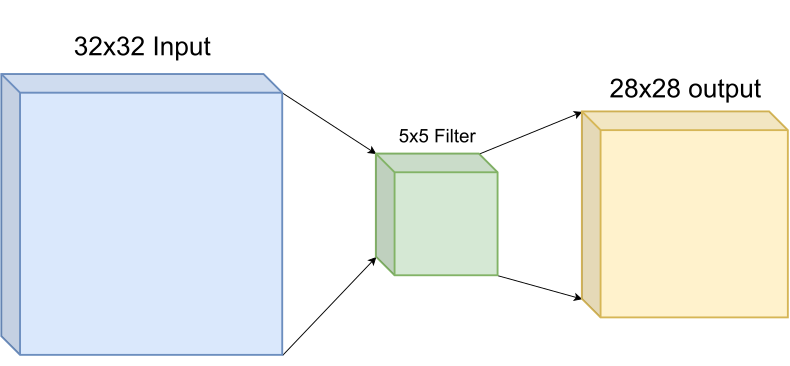
\includegraphics[keepaspectratio, scale=0.25]{pic/Padding2.png}
		\smallskip
		\small 32x32 input shrinks to 28x28 output. (information loss occurs)
	\end{frame}
	\begin{frame}{Solution?}
		\begin{center}
			\LARGE What is the solution?
		\end{center}
	\end{frame}
	\begin{frame}{Padding}
		\begin{center}
			\LARGE \textbf{Padding}: the secret ingredient to keep strides in line!
		\end{center}
	\end{frame}
	\begin{frame}{Padding}
		
		\begin{minipage}{0.28\textwidth} % Adjust width to your liking
			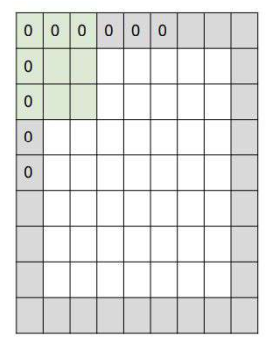
\includegraphics[keepaspectratio, scale=0.6]{pic/zeropad.png}
		\end{minipage}
		\begin{minipage}{0.67\textwidth} % Adjust width to your liking
			In practice, it is common to zero-pad the border. \\
			\smallskip
			\textbf{Recall:}The original formula for convolution without padding:
			\[
			\frac{N - F}{\text{stride}} + 1
			\]
			
			Now, we should adjust the formula considering padding $P$:
			\[
			\frac{N + 2P - F}{\text{stride}} + 1
			\]
		\end{minipage}
		
		\vfill
		\begin{tikzpicture}[remember picture,overlay]
			\node[anchor=south west, xshift=0.5cm, yshift=0.5cm] at (current page.south west) {
				\scriptsize Figure adapted from [2]
			};
		\end{tikzpicture}
	\end{frame}
	\begin{frame}{Padding}
		\begin{itemize}
			\item Zero-padding is used not only for stride $> 1$, but also \textbf{to prevent a reduction} in output size even when $S = 1$.
			
			\item For stride $> 1$, zero padding is adjusted to ensure that the size of the convolved output is: $\left\lceil \frac{N}{S} \right\rceil$
			\\
			This is achieved by zero padding the image with:  $ P = S\left\lceil \frac{N}{S} \right\rceil - N$
			
			\item For an $F$ width filter:
			\begin{itemize}
				\item \textbf{Odd $F$}: Pad on both left and right with $\frac{F-1}{2}$ columns of zeros.
				\item \textbf{Even $F$}: Pad one side with $\frac{F}{2}$ columns of zeros, and the other with $\frac{F}{2} - 1$ columns of zeros.
				\item The resulting image is width: \textbf{$N + F - 1$}
			\end{itemize}
			\item The top \& bottom zero padding follows the same rules to maintain map height after convolution.
			
		\end{itemize}
	\end{frame}
	\begin{frame}{Convnet}
		\centering
		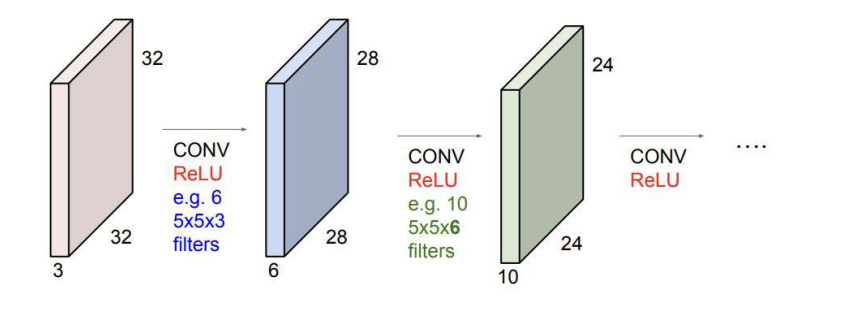
\includegraphics[keepaspectratio, scale=0.7]{pic/convnet.png}
		\smallskip
		\begin{itemize}
			\item \textbf {ConvNet:} a sequence of convolution layers \textbf{interspersed with activation functions.}
		\end{itemize}
		
		\vfill
		\begin{tikzpicture}[remember picture,overlay]
			\node[anchor=south west, xshift=0.5cm, yshift=0.5cm] at (current page.south west) {
				\scriptsize Figure adapted from [2]
			};
		\end{tikzpicture}
	\end{frame}
	\begin{frame}{Convnet}
		\textbf{Question:}
		What do convolutional filters at different levels of a ConvNet learn?
	\end{frame}
	\begin{frame}{Convnet}
		\textbf{Question:}
		What do convolutional filters at different levels of a ConvNet learn?
		
		\bigskip
		
		\textbf{Answer:}
		\begin{itemize}
			\item Filters in the \textbf{early layers} typically detect \textbf{simple features} such as edges, textures, and basic shapes.
			\item As we move \textbf{deeper} into the network, the filters learn \textbf{more complex and abstract features}, such as specific parts of objects (e.g., a nose, eyes, or other high-level patterns).
		\end{itemize}
	\end{frame}
	
	\begin{frame}{Convolution Output}
		\begin{itemize}
			\item Accepts a volume of size $W_1 \times H_1 \times D_1$
			\item Requires four hyper-parameters:
			\begin{itemize}
				\item Number of filters $K$
				\item Their spatial extent $F$
				\item The stride $S$
				\item The amount of zero padding $P$
			\end{itemize}
			
			\item Produces a volume of size $W_2 \times H_2 \times D_2$ where:
			\begin{itemize}
				\item $W_2 = \left( \frac{W_1 - F + 2P}{S} \right) + 1$
				\item $H_2 = \left( \frac{H_1 - F + 2P}{S} \right) + 1$
				\vspace{2pt}
				\item $D_2 = K$
			\end{itemize}
		\end{itemize}
		
	\end{frame}
	\begin{frame}{Parameter Setting}
		
		
		\begin{minipage}{0.50\textwidth} % Left side for general info
			\begin{itemize}
				\item With parameter sharing, convolution introduces $F \cdot F \cdot D_1$ weights per filter, for a total of $(F \cdot F \cdot D_1) \cdot K$ weights and $K$ biases.
			\end{itemize}
		\end{minipage}
		\hfill % Horizontal space between the two minipages
		\begin{minipage}{0.45\textwidth} % Right side for common settings
			\textbf{Common settings:}
			\begin{itemize}
				\item $K =$ powers of 2 (e.g., 32, 64, \dots)
				\item $F = 3$, $S = 1$, $P = 1$
				\item $F = 5$, $S = 1$, $P = 2$
				\item $F = 5$, $S = 2$, $P = $ adjusted accordingly.
				\item $F = 1$, $S = 1$, $P = 0$
			\end{itemize}
		\end{minipage}
	\end{frame}
	
	\begin{frame}{Example}
		\textbf{Question:}
		Given an input volume of \textcolor{blue}{32x32x3}, we apply \textcolor{red}{10} filters, each of size \textcolor{purple}{5x5}, with a stride of \textcolor{deepgreen}{1} and padding of \textcolor{purple}{2}.\\[10pt]
		
		\begin{itemize}
			\item What is the output volume size of this convolutional layer?
			\item How many parameters are required for this convolutional layer?
		\end{itemize}
		
	\end{frame}
	
	\begin{frame}{Example}
		
		\textbf{Output Volume Size:}\\
		\[
		\left(\frac{32 + 2 \times 2 - 5}{1}\right) + 1 = 32 \quad \text{(spatial dimensions)}, \quad \textcolor{blue}{32 \times 32 \times} \textcolor{red}{10}
		\]
		
		\bigskip
		\textbf{Number of Parameters:}\\
		\bigskip
		
		Each filter parameters: \(5 \times 5 \times 3 + 1 = 76\) \hspace{15pt} \textit{(+1 for bias)}.\\
		Therefore, total parameters: \(76 \times 10 = \textbf{760}\).
		
	\end{frame}
	
	\section{Backpropagation}
	
	
	\begin{frame}{Example Overview}
		\begin{itemize}
			\item we will tackle this problem with an example using stride = 2 and padding = 0.
		\end{itemize}
		\centering
		\includegraphics[keepaspectratio, scale=0.28]{pic/BP1.png}
		
				\vfill
		\begin{tikzpicture}[remember picture,overlay]
			\node[anchor=south west, xshift=0.5cm, yshift=0.5cm] at (current page.south west) {
				\scriptsize Figures adapted from [7]
			};
		\end{tikzpicture}
	\end{frame}
	
	\begin{frame}{Convolution}
		\centering
		\large \textbf{Recall}: convolution process
	\end{frame}
	\begin{frame}{Convolution}
		\centering
		\includegraphics[keepaspectratio, scale=0.3]{pic/BP2.png}
	\end{frame}
	
	\begin{frame}{Convolution}
		\centering
		\includegraphics[keepaspectratio, scale=0.3]{pic/BP3.png}
	\end{frame}
	
	\begin{frame}{Convolution}
		\centering
		\includegraphics[keepaspectratio, scale=0.3]{pic/BP4.png}
	\end{frame}
	
	\begin{frame}{Convolution}
		\centering
		\includegraphics[keepaspectratio, scale=0.3]{pic/BP5.png}
	\end{frame}
	
	\begin{frame}{Another view}
		\begin{align*}
			z_1 &= w_1 \times a_1 + w_2 \times a_2 + w_3 \times a_3 + w_4 \times a_4 + + \cdots + w_9 \times a_{13} \\
			z_2 &= w_1 \times a_3 + w_2 \times a_4 + w_3 \times a_5 + w_4 \times a_8 + \cdots + w_9 \times a_{15} \\
			z_3 &= w_1 \times a_{11} + w_2 \times a_{12} + w_3 \times a_{13} + w_4 \times a_{16} + \cdots + w_9 \times a_{23} \\
			z_4 &= w_1 \times a_{13} + w_2 \times a_{14} + w_3 \times a_{15} + w_4 \times a_{18} + \cdots + w_9 \times a_{25}
		\end{align*}
	\end{frame}
	
	\begin{frame}{Whole Network}
		\begin{itemize}
			\item For easier computation, we will assume one layer of convolution and a perceptron as our whole network.
			\item \textbf{Recall}: \(w_i^* = w_i - \alpha \times \frac{\partial L}{\partial w_i}\)
		\end{itemize}
		\smallskip
		\centering
		\includegraphics[keepaspectratio, scale=0.25]{pic/BP6.png}
	\end{frame}
	
	
	\begin{frame}{Gradient}
		\begin{itemize}
			\item We can easily calculate the gradients:  
		\end{itemize}
		\smallbreak
		\begin{align*}
			\frac{\partial L}{\partial w_1} &= \frac{\partial z_1}{\partial w_1} \frac{\partial L}{\partial z_1} + \frac{\partial z_2}{\partial w_1} \frac{\partial L}{\partial z_2} + \frac{\partial z_3}{\partial w_1} \frac{\partial L}{\partial z_3} + \frac{\partial z_4}{\partial w_1} \frac{\partial L}{\partial z_4} \\
			&= a_1 \frac{\partial L}{\partial z_1} + a_3 \frac{\partial L}{\partial z_2} + a_{11} \frac{\partial L}{\partial z_3} + a_{13} \frac{\partial L}{\partial z_4}
		\end{align*}
		
	\end{frame}
	
	\begin{frame}{Gradient}
		\centering \large \textbf{Do the same for each $w$}
	\end{frame}
	
	\begin{frame}
		\begin{align*}
			\frac{\partial L}{\partial w_1} &= a_1 \frac{\partial L}{\partial z_1} + a_3 \frac{\partial L}{\partial z_2} + a_{11} \frac{\partial L}{\partial z_3} + a_{13} \frac{\partial L}{\partial z_4} \\
			\frac{\partial L}{\partial w_2} &= a_2 \frac{\partial L}{\partial z_1} + a_4 \frac{\partial L}{\partial z_2} + a_{12} \frac{\partial L}{\partial z_3} + a_{14} \frac{\partial L}{\partial z_4} \\
			\frac{\partial L}{\partial w_3} &= a_3 \frac{\partial L}{\partial z_1} + a_5 \frac{\partial L}{\partial z_2} + a_{13} \frac{\partial L}{\partial z_3} + a_{15} \frac{\partial L}{\partial z_4} \\
			\frac{\partial L}{\partial w_4} &= a_6 \frac{\partial L}{\partial z_1} + a_8 \frac{\partial L}{\partial z_2} + a_{16} \frac{\partial L}{\partial z_3} + a_{18} \frac{\partial L}{\partial z_4} \\
			\frac{\partial L}{\partial w_5} &= a_7 \frac{\partial L}{\partial z_1} + a_9 \frac{\partial L}{\partial z_2} + a_{17} \frac{\partial L}{\partial z_3} + a_{19} \frac{\partial L}{\partial z_4} \\...
		\end{align*}
		
	\end{frame}
	\begin{frame}{Overview}
		\centering
		\includegraphics[keepaspectratio, scale=0.15]{pic/BP11.png}
	\end{frame}
	\begin{frame}{Result}
		\centering
		\includegraphics[keepaspectratio, scale=0.45]{pic/BP12.png}
	\end{frame}
	
	
	\begin{frame}{What's next?}
		\centering \large \textbf{Proceed with gradient descent.}
	\end{frame}
	
	\begin{frame}{So Far}
		
		\begin{itemize}
			\item The highly structured nature of image data.
			\item Local correlations are important.
			\item CNNs have local and shared connections.
			\item Strides \& padding.
		\end{itemize}
		
	\end{frame}
	
	\begin{frame}{Up Next}
		
		\centering \large \textbf{Learn more details about CNNs!}
		
	\end{frame}
	
	
	
	\section{References}
	
	\begin{frame}{Contributions}
		\begin{itemize}
			\item \textbf{This slide has been prepared thanks to:}
			\begin{itemize}
				\setlength{\itemsep}{10pt}
				\item \href{https://github.com/Ali0281}{Ali Aghayari}
			\end{itemize}
		\end{itemize}
		
	\end{frame}
	
	\begin{frame}[allowframebreaks]
		\bibliography{ref}
		\bibliographystyle{ieeetr}
		\nocite{*}
	\end{frame}
	
	
	
	
\end{document}